\clearpage
\appendix

\def\thesection{付録\Alph{section}}
\renewcommand{\thetable}{\Alph{section}.\arabic{table}}
\renewcommand{\thefigure}{\Alph{section}.\arabic{figure}}


\section{使用したモデルのパラメータの意味}\label{paramMean}
本付録では,使用したモデルのパラメータの意味について名前としてある程度整備されているが,実際の入力でどのように変化するのかを示す.
図\ref{fig:cakeParamMean_1} - \ref{fig:cakeParamMean_4}に
Cake モデルにおいての,図\ref{fig:sofaParamMean_1} - \ref{fig:sofaParamMean_7}に Sofa モデルにおいてのパラメータが最小と最大の時のモデルを示す.

\begin{figure}[h]
 \begin{minipage}[b]{0.48\linewidth}
  \centering
  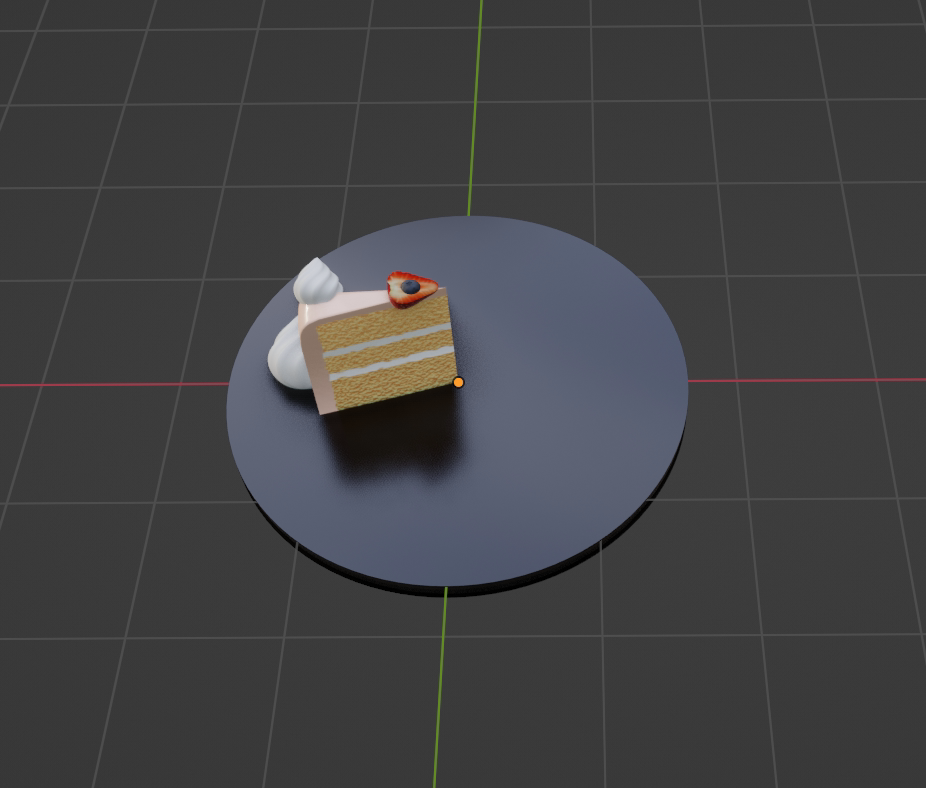
\includegraphics[scale=0.25]{./imgs/cakeParamMean/cutMin.png}
        \subcaption{Cake cut 最小(0.0)}
 \end{minipage}
 \begin{minipage}[b]{0.48\linewidth}
  \centering
  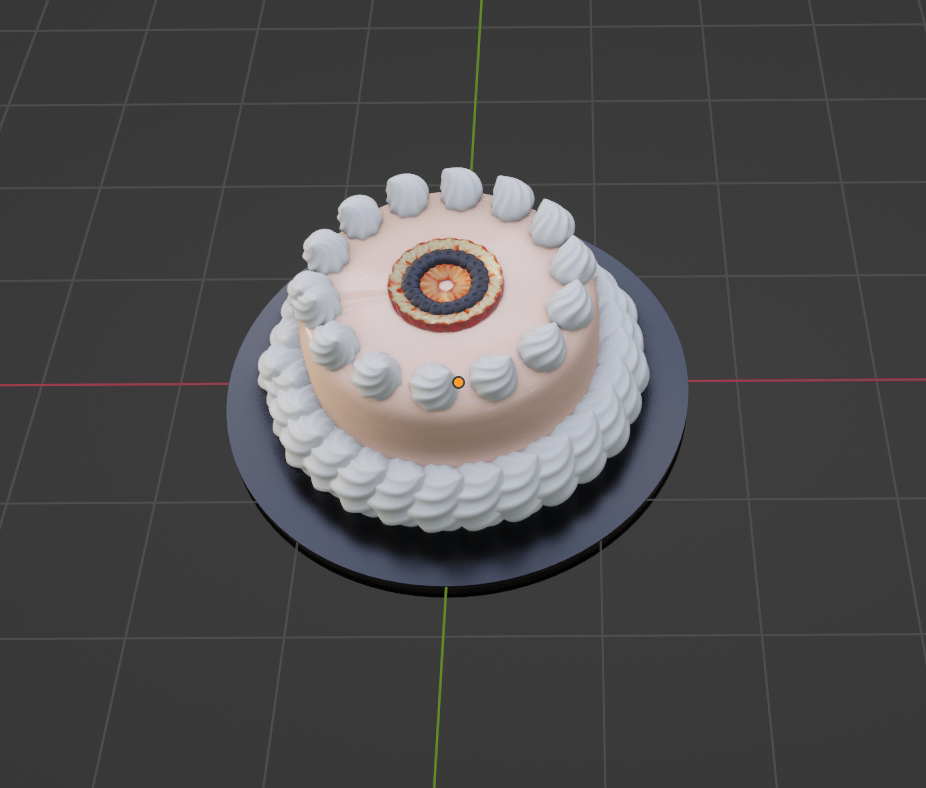
\includegraphics[scale=0.25]{./imgs/cakeParamMean/cutMax.png}
        \subcaption{Cake cut 最大(1.0)}
 \end{minipage}\\
 \begin{minipage}[b]{0.48\linewidth}
  \centering
  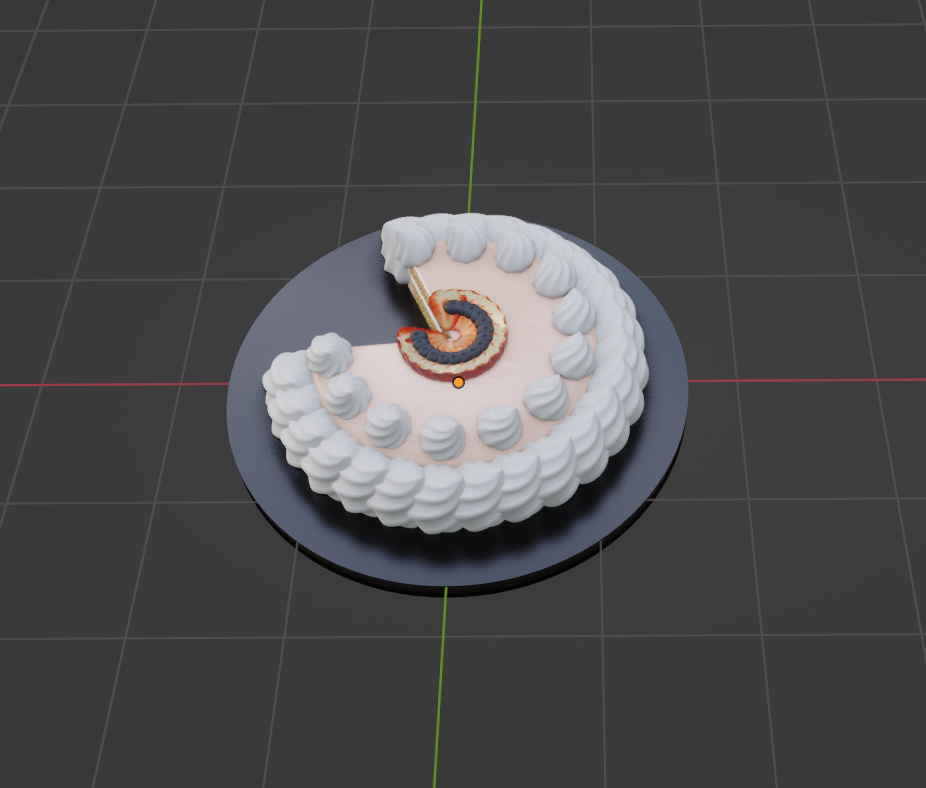
\includegraphics[scale=0.25]{./imgs/cakeParamMean/heightMin.png}
        \subcaption{Cake height 最小(0.5)}
 \end{minipage}
 \begin{minipage}[b]{0.48\linewidth}
  \centering
  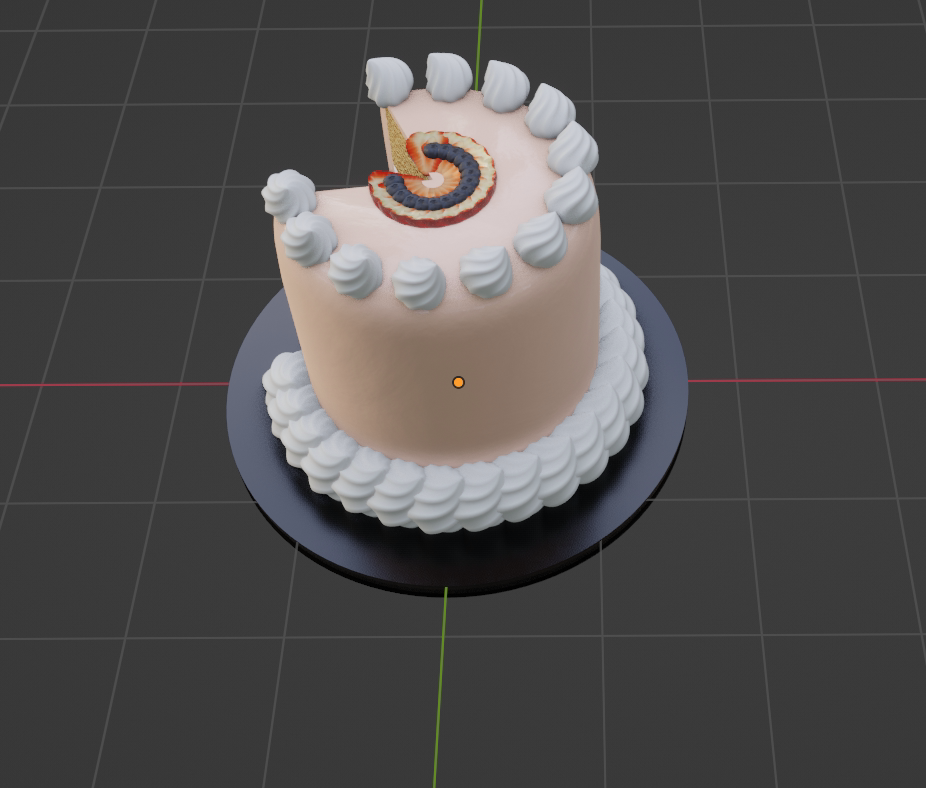
\includegraphics[scale=0.25]{./imgs/cakeParamMean/heightMax.png}
        \subcaption{Cake height 最大(2.0)}
 \end{minipage}
 \caption{Cake モデルにおけるパラメータ範囲(1)}\label{fig:cakeParamMean_1}
\end{figure}

\begin{figure}[h]
 \begin{minipage}[b]{0.48\linewidth}
  \centering
  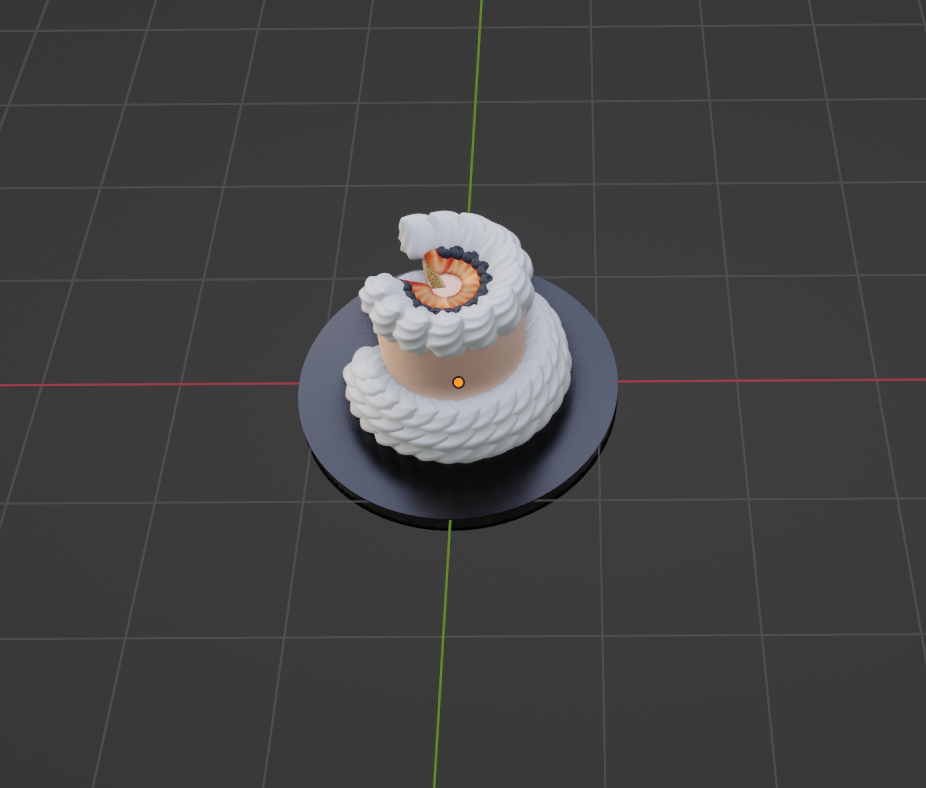
\includegraphics[scale=0.25]{./imgs/cakeParamMean/radiusMin.png}
        \subcaption{Cake radius 最小(0.0)}
 \end{minipage}
 \begin{minipage}[b]{0.48\linewidth}
  \centering
  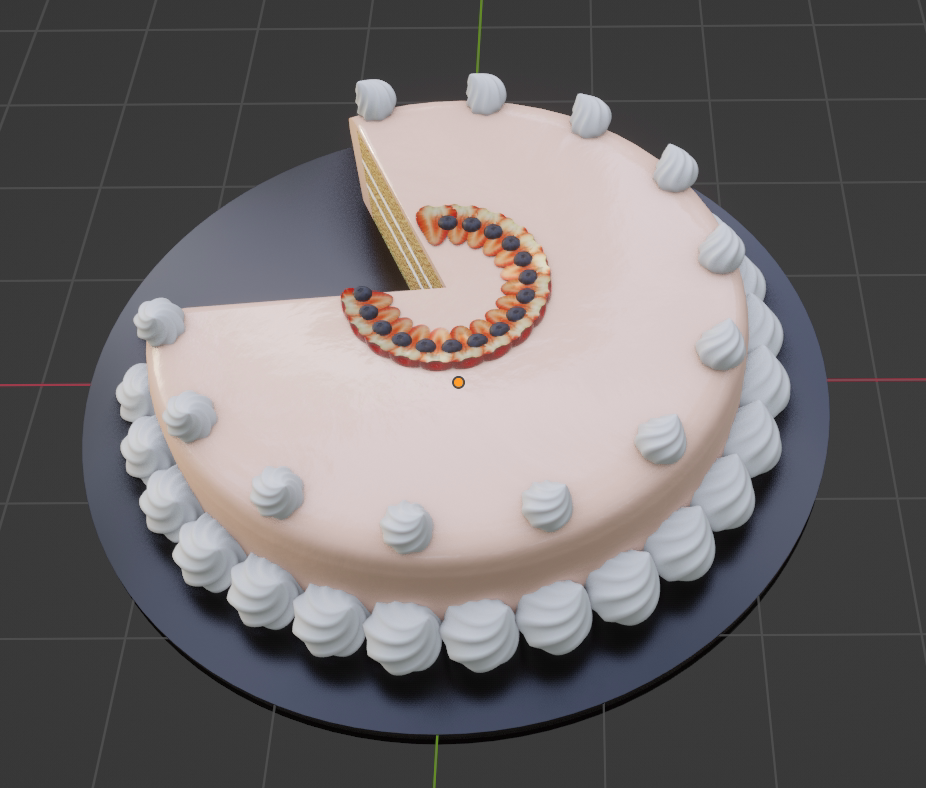
\includegraphics[scale=0.25]{./imgs/cakeParamMean/radiusMax.png}
        \subcaption{Cake radius 最大(1.0)}
 \end{minipage}\\
  \begin{minipage}[b]{0.48\linewidth}
  \centering
  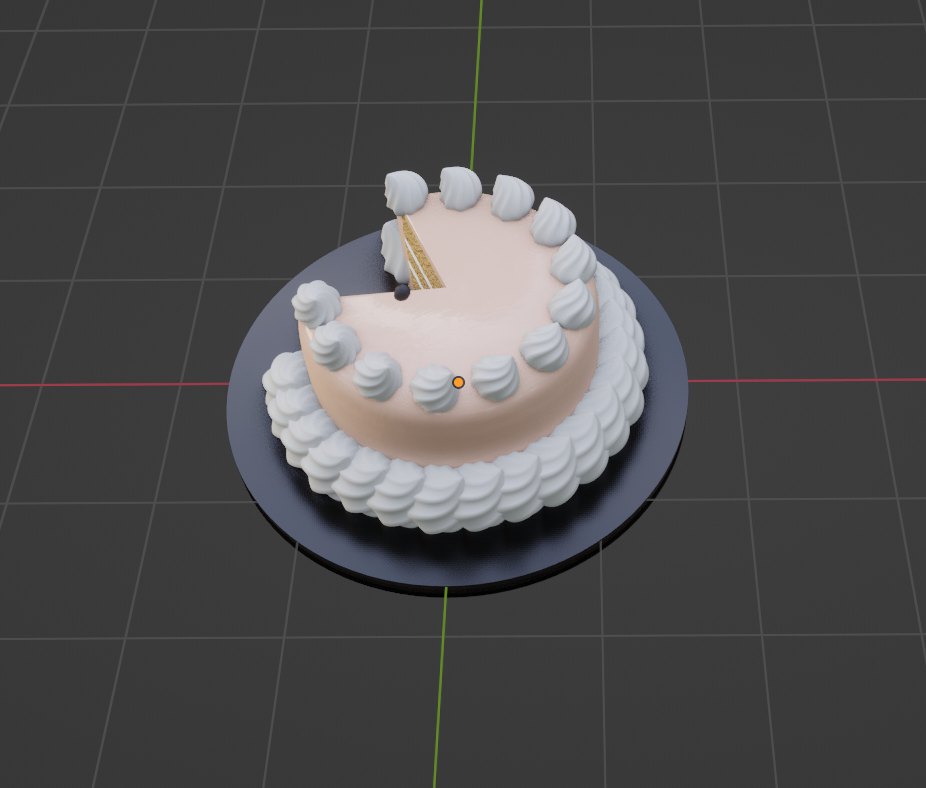
\includegraphics[scale=0.25]{./imgs/cakeParamMean/toppingQuanMin.png}
        \subcaption{Topping quantity 最小(0.0)}
 \end{minipage}
 \begin{minipage}[b]{0.48\linewidth}
  \centering
  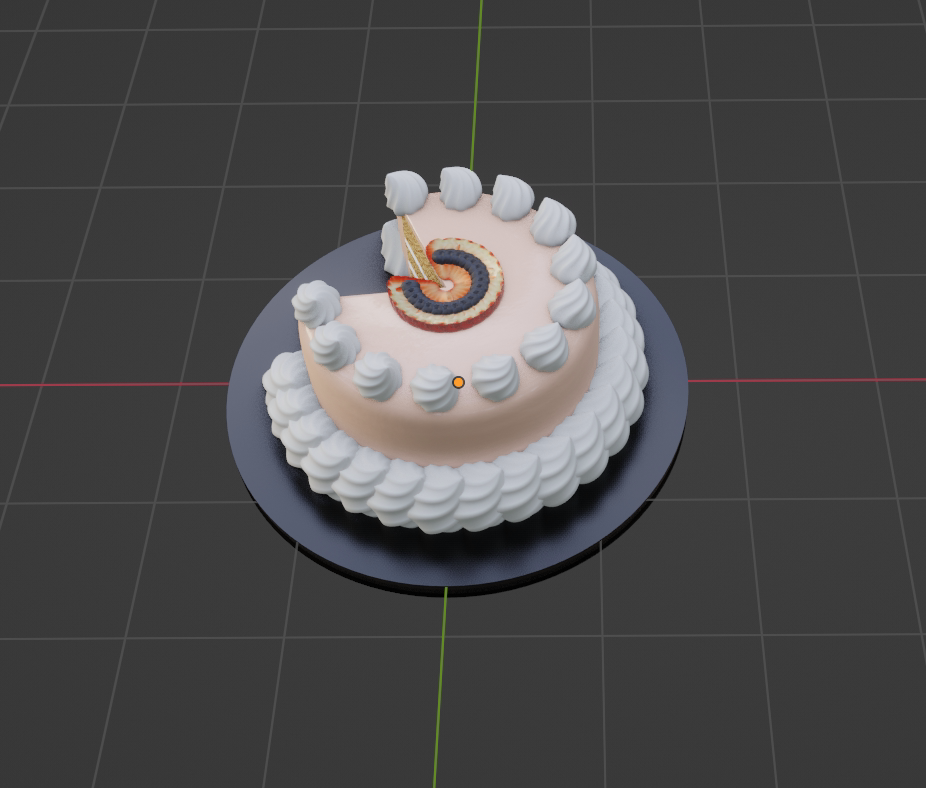
\includegraphics[scale=0.25]{./imgs/cakeParamMean/toppingQuanMax.png}
        \subcaption{Topping quantity 最大(50.0)}
 \end{minipage}\\
 \begin{minipage}[b]{0.48\linewidth}
  \centering
  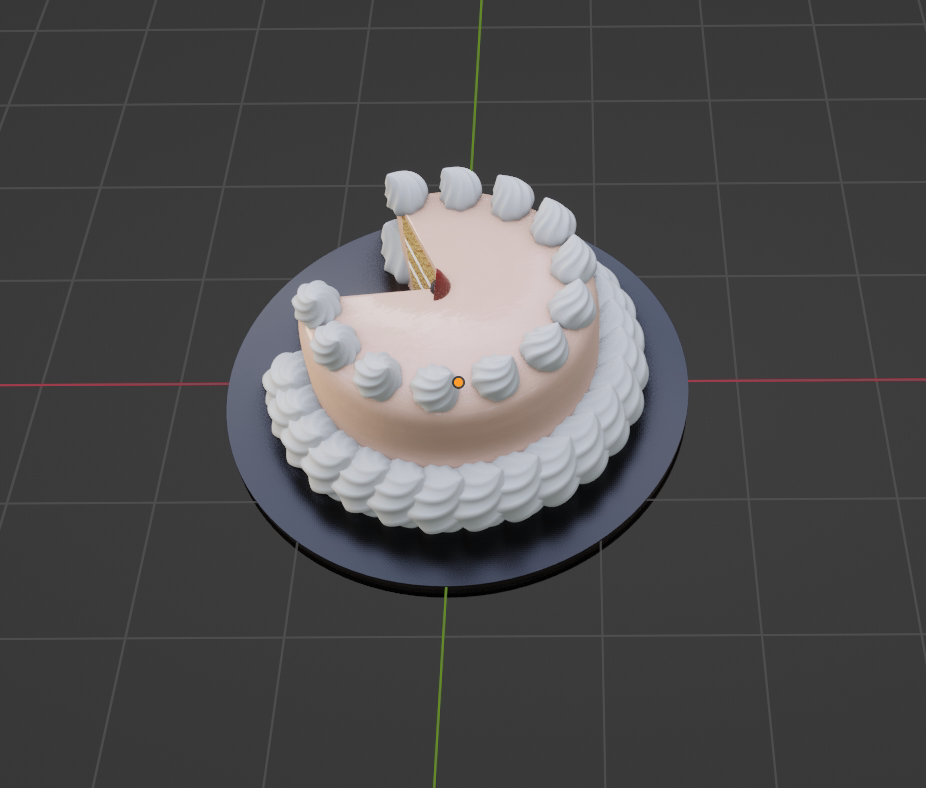
\includegraphics[scale=0.25]{./imgs/cakeParamMean/toppingPosMin.png}
        \subcaption{Topping position 最小(0.0)}
 \end{minipage}
 \begin{minipage}[b]{0.48\linewidth}
  \centering
  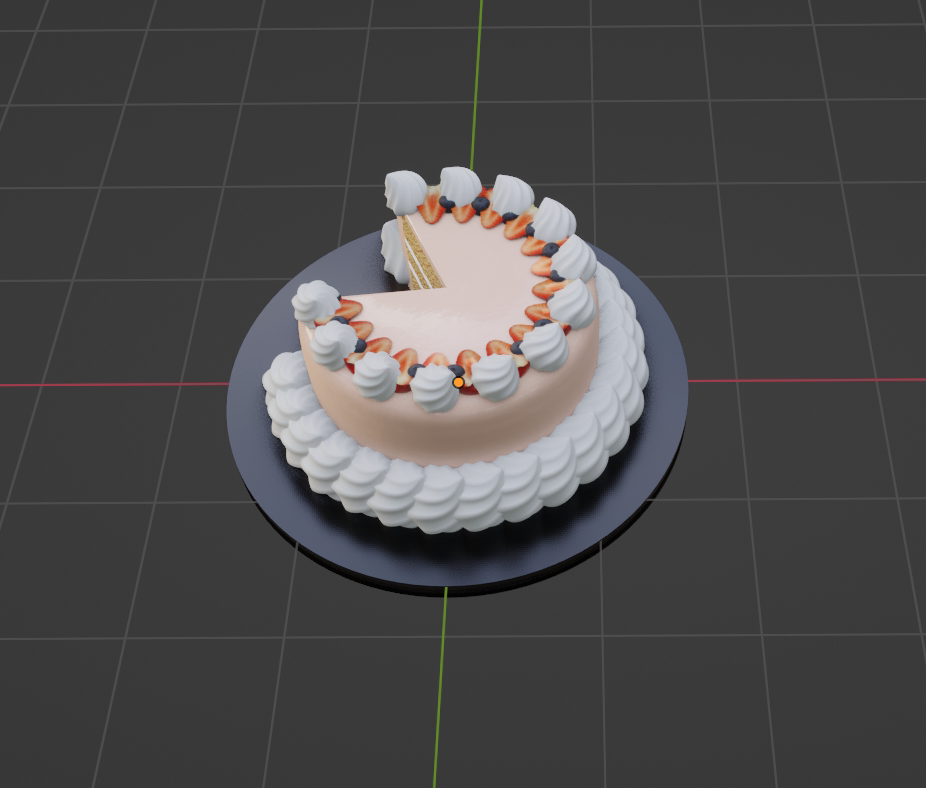
\includegraphics[scale=0.25]{./imgs/cakeParamMean/toppingPosMax.png}
        \subcaption{Topping position 最大(1.0)}
 \end{minipage}
 \caption{Cake モデルにおけるパラメータ範囲(2)}\label{fig:cakeParamMean_2}
\end{figure}

\begin{figure}[h]
 \begin{minipage}[b]{0.48\linewidth}
  \centering
  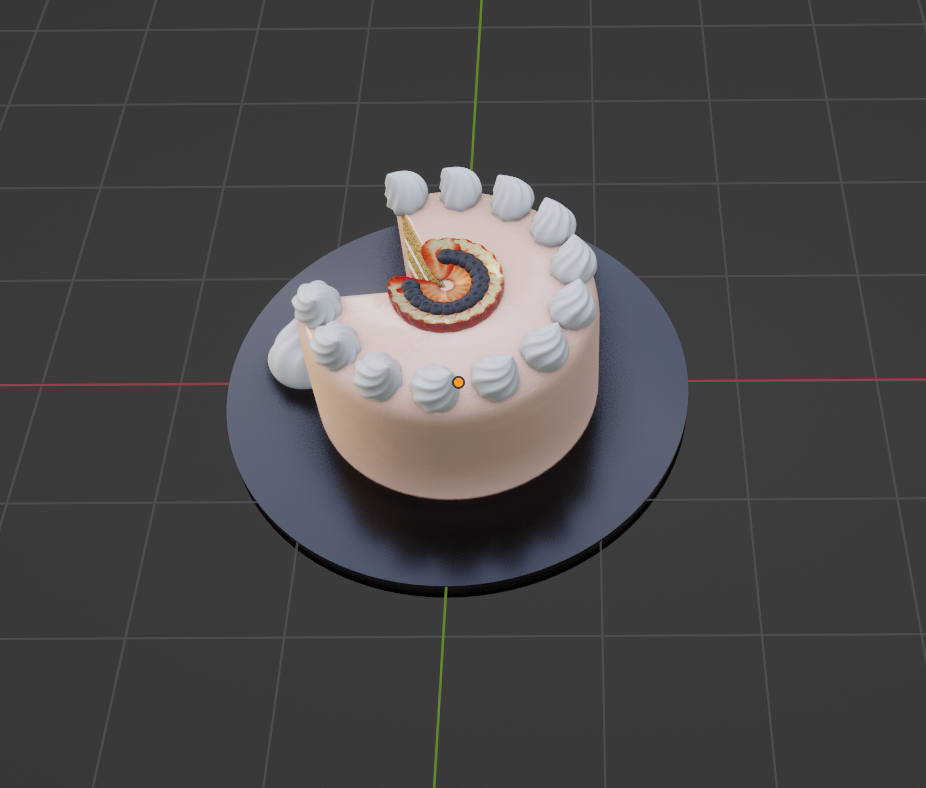
\includegraphics[scale=0.25]{./imgs/cakeParamMean/botQuanMin.png}
        \subcaption{CreamBot quantity 最小(0.0)}
 \end{minipage}
 \begin{minipage}[b]{0.48\linewidth}
  \centering
  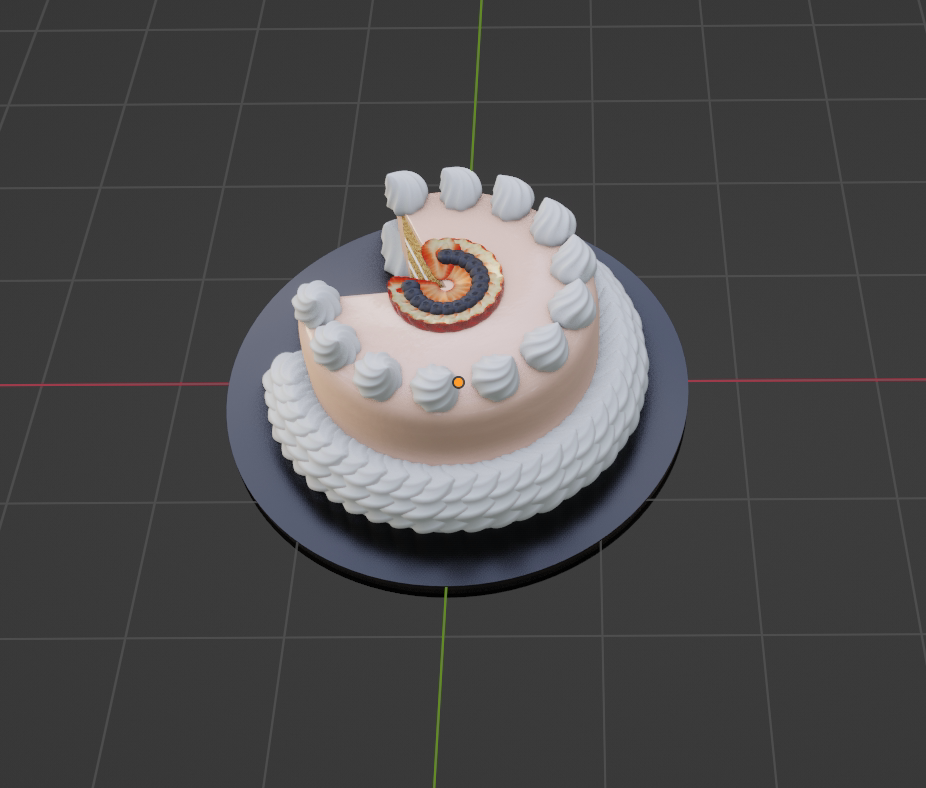
\includegraphics[scale=0.25]{./imgs/cakeParamMean/botQuanMax.png}
        \subcaption{CreamBot quantity 最大(50.0)}
 \end{minipage}\\
  \begin{minipage}[b]{0.48\linewidth}
  \centering
  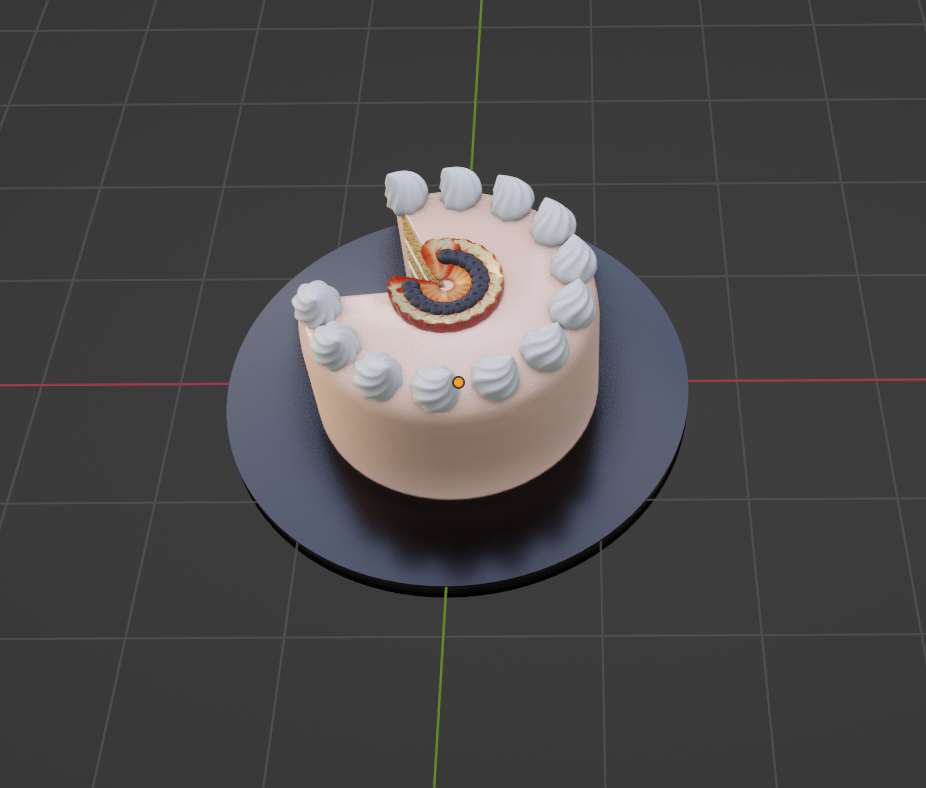
\includegraphics[scale=0.25]{./imgs/cakeParamMean/botSizeMin.png}
        \subcaption{CreamBot size 最小(0.0)}
 \end{minipage}
 \begin{minipage}[b]{0.48\linewidth}
  \centering
  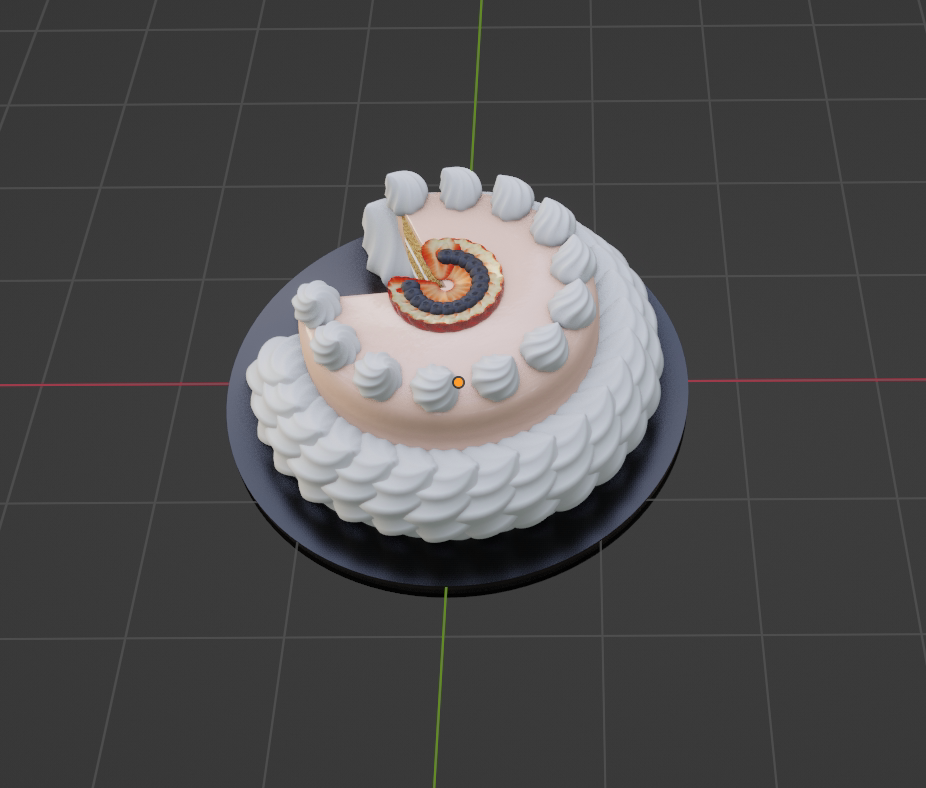
\includegraphics[scale=0.25]{./imgs/cakeParamMean/botSizeMax.png}
        \subcaption{CreamBot size 最大(2.0)}
 \end{minipage}\\
 \begin{minipage}[b]{0.48\linewidth}
  \centering
  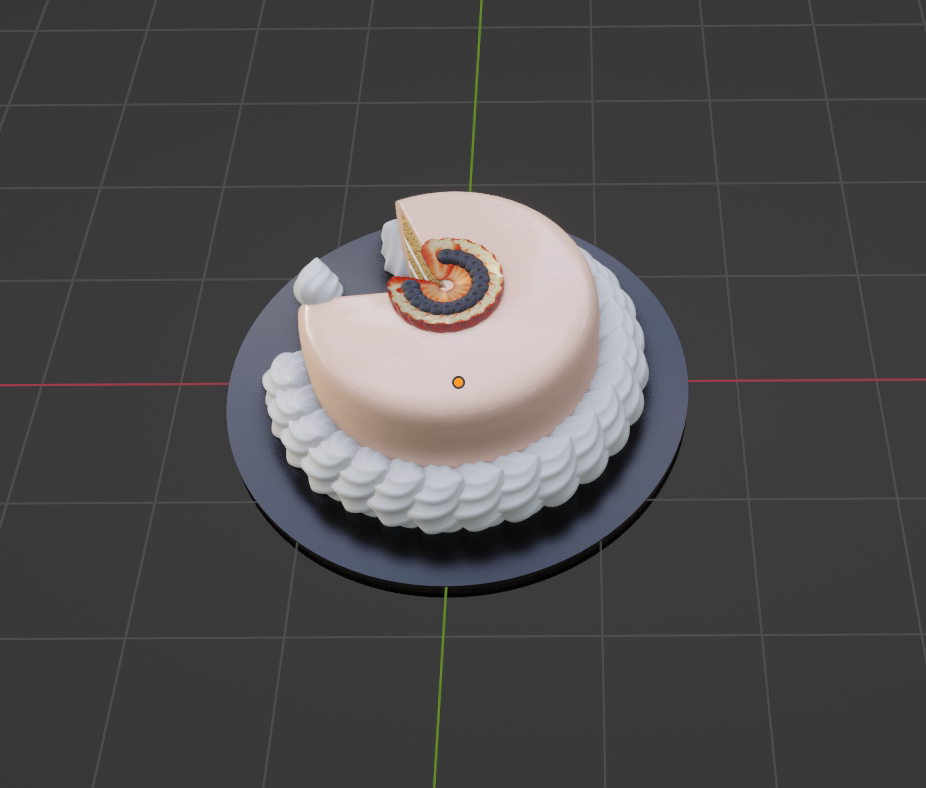
\includegraphics[scale=0.25]{./imgs/cakeParamMean/topQuanMin.png}
        \subcaption{CreamTop quantity 最小(0.0)}
 \end{minipage}
 \begin{minipage}[b]{0.48\linewidth}
  \centering
  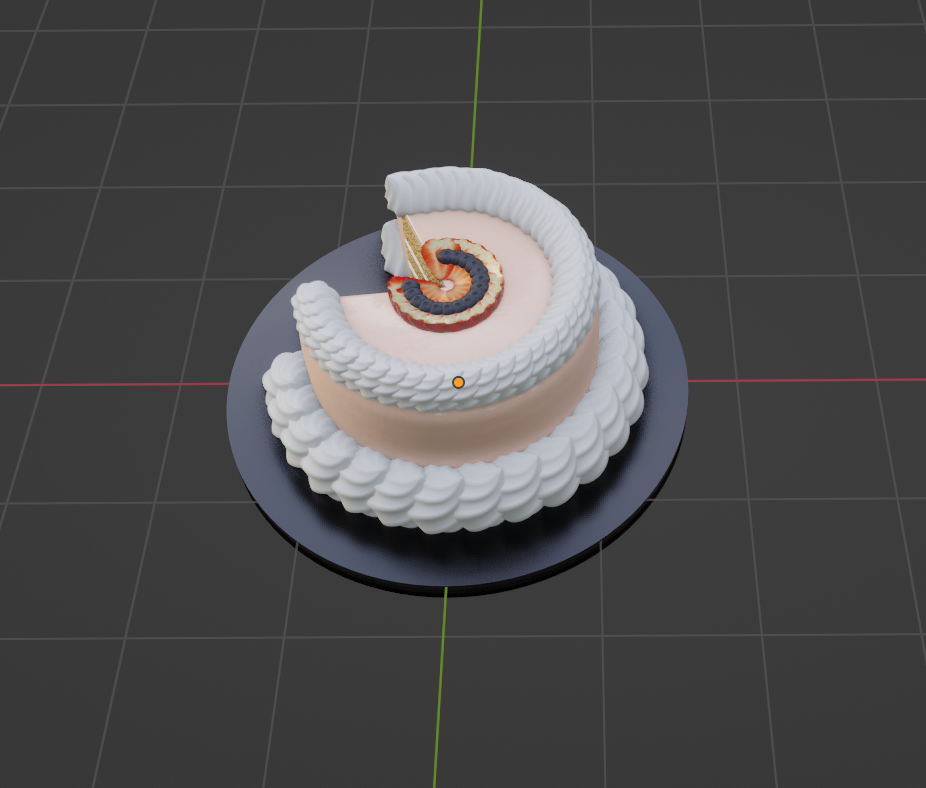
\includegraphics[scale=0.25]{./imgs/cakeParamMean/topQuanMax.png}
        \subcaption{CreamTop quantity 最大(50.0)}
 \end{minipage}
 \caption{Cake モデルにおけるパラメータ範囲(3)}\label{fig:cakeParamMean_3}
\end{figure}


\begin{figure}[h]
 \begin{minipage}[b]{0.48\linewidth}
  \centering
  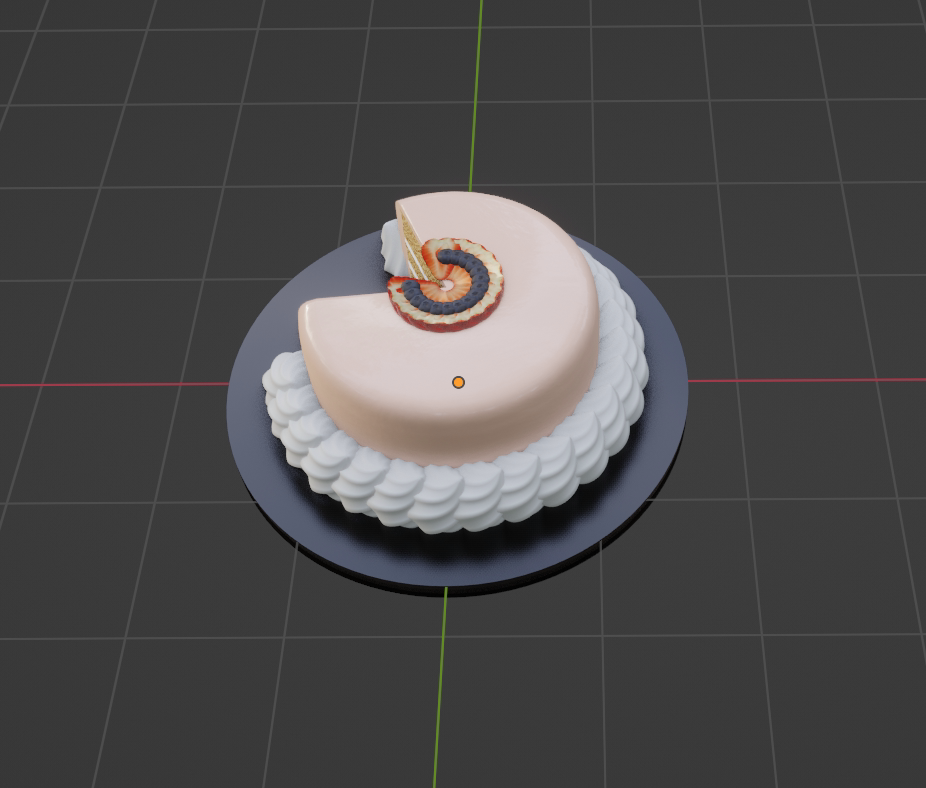
\includegraphics[scale=0.25]{./imgs/cakeParamMean/topSizeMin.png}
        \subcaption{CreamTop size 最小(0.0)}
 \end{minipage}
 \begin{minipage}[b]{0.48\linewidth}
  \centering
  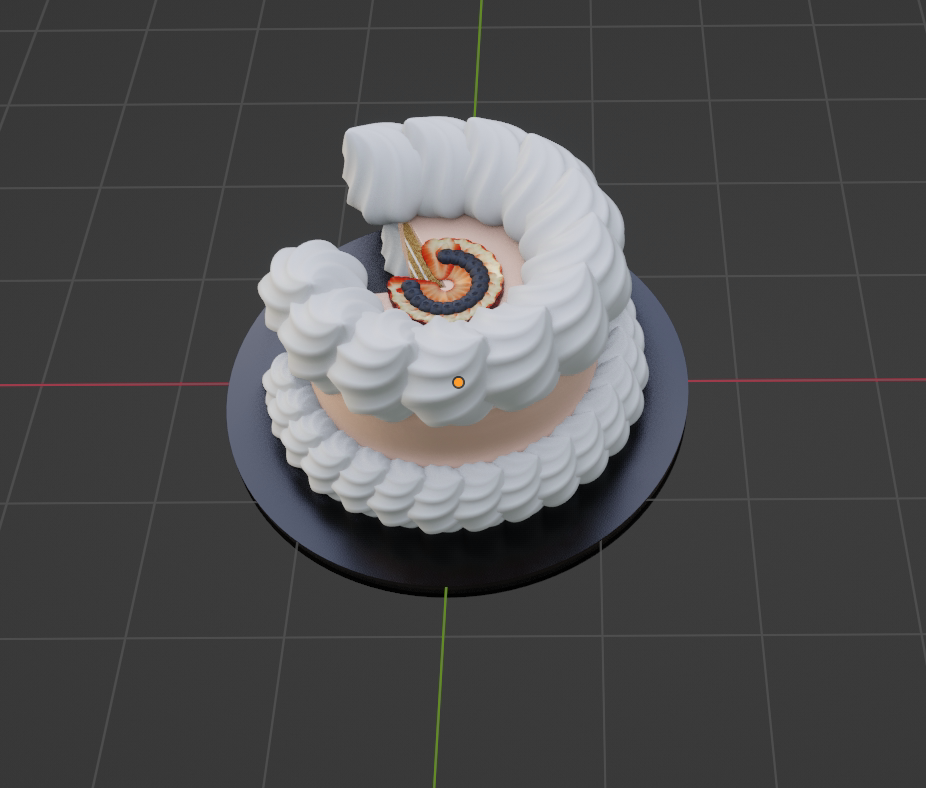
\includegraphics[scale=0.25]{./imgs/cakeParamMean/topSizeMax.png}
        \subcaption{CreamTop size 最大(2.0)}
 \end{minipage}\\
 \begin{minipage}[b]{0.48\linewidth}
  \centering
  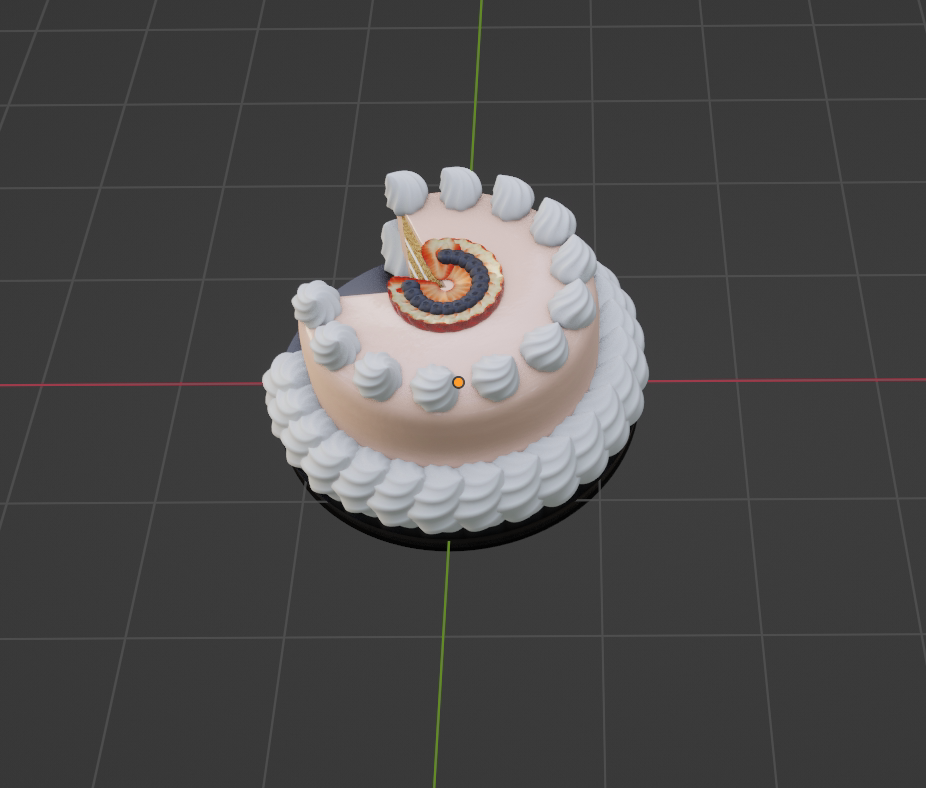
\includegraphics[scale=0.25]{./imgs/cakeParamMean/plateSizeMin.png}
        \subcaption{Plate size 最小(0.3)}
 \end{minipage}
 \begin{minipage}[b]{0.48\linewidth}
  \centering
  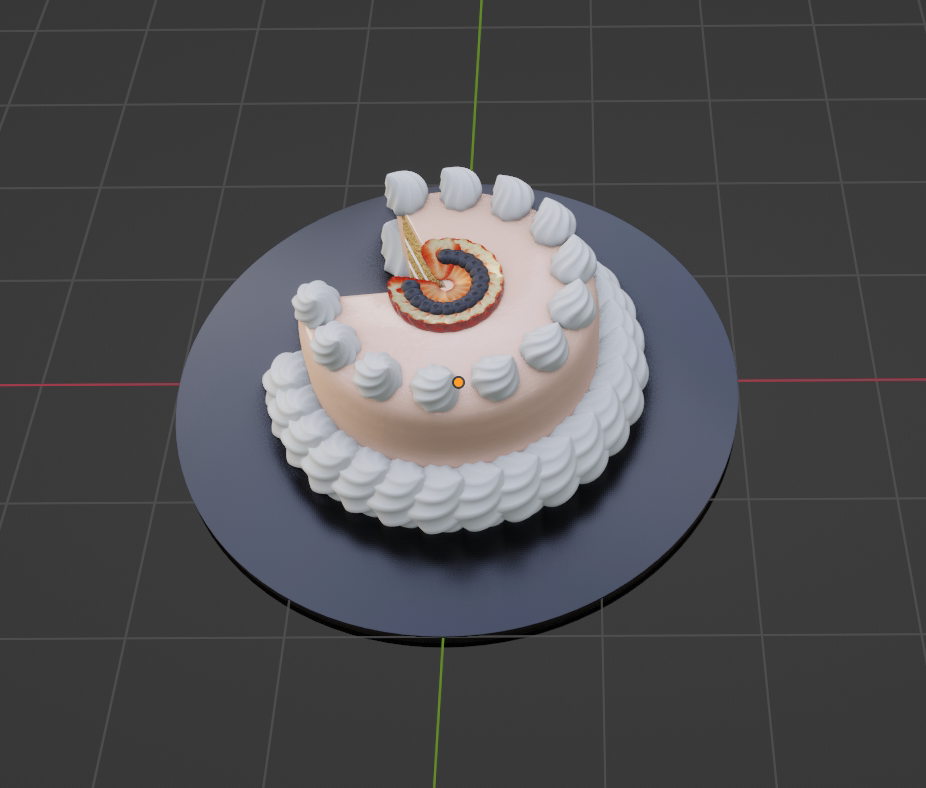
\includegraphics[scale=0.25]{./imgs/cakeParamMean/plateSizeMax.png}
        \subcaption{Plate size 最大(1.0)}
 \end{minipage}\\
 \begin{minipage}[b]{0.48\linewidth}
  \centering
  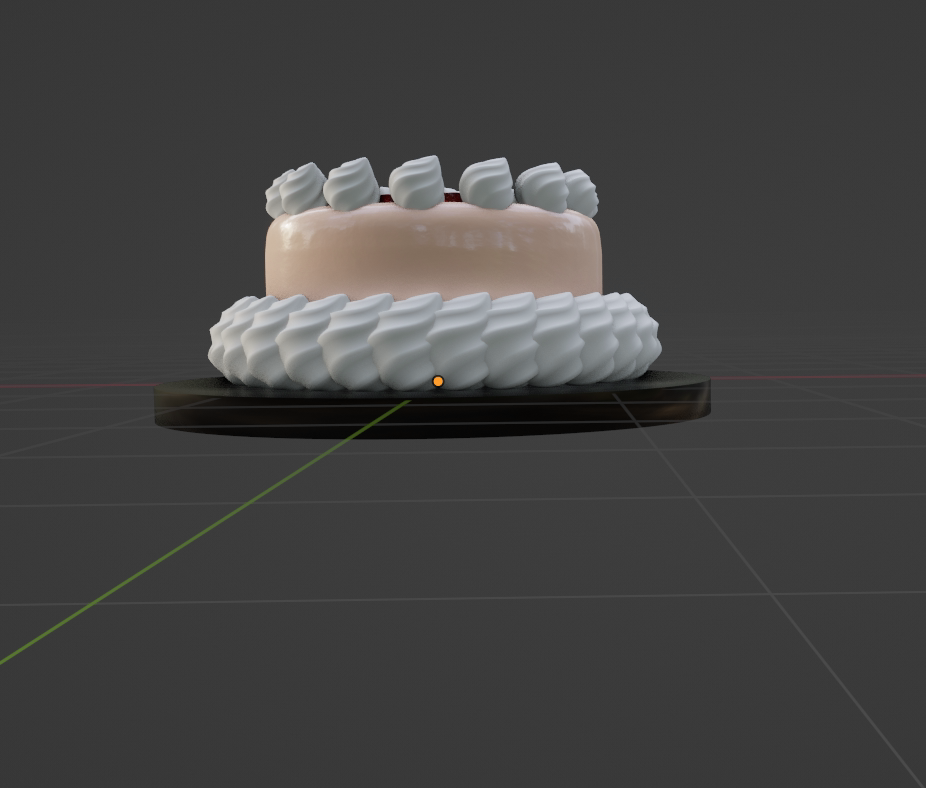
\includegraphics[scale=0.25]{./imgs/cakeParamMean/tickMin.png}
        \subcaption{Plate thickness 最小(-0.2)}
 \end{minipage}
 \begin{minipage}[b]{0.48\linewidth}
  \centering
  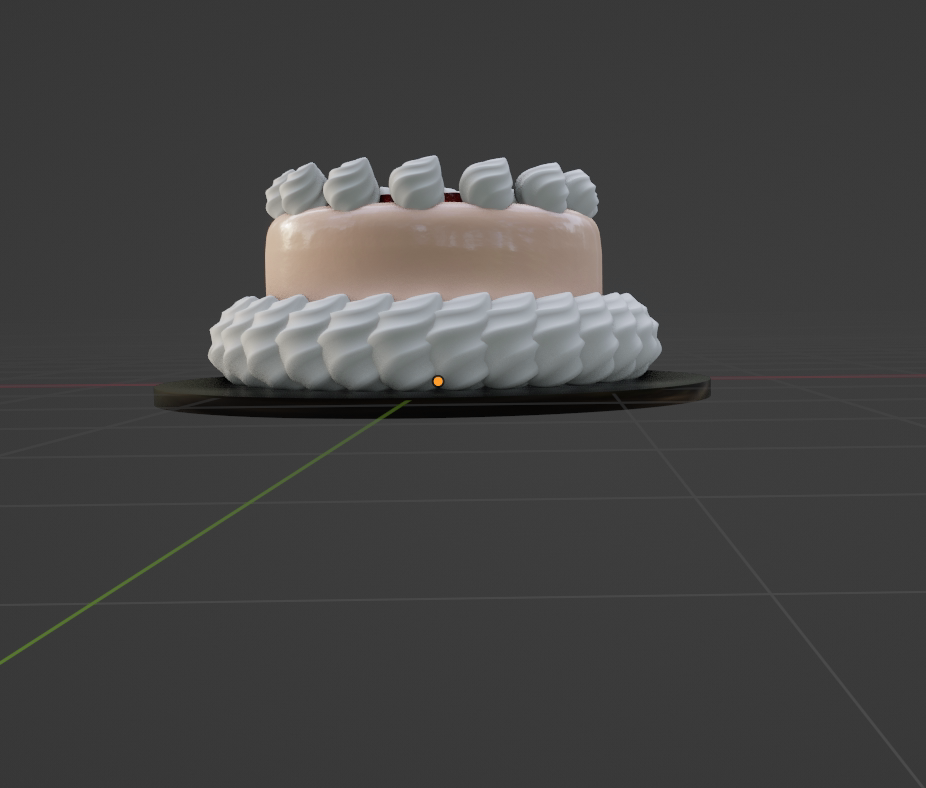
\includegraphics[scale=0.25]{./imgs/cakeParamMean/tickMax.png}
        \subcaption{Plate thickness 最大(-0.1)}
 \end{minipage}
 \caption{Cake モデルにおけるパラメータ範囲(4)}\label{fig:cakeParamMean_4}
\end{figure}
\begin{figure}[h]
 \begin{minipage}[b]{0.48\linewidth}
  \centering
  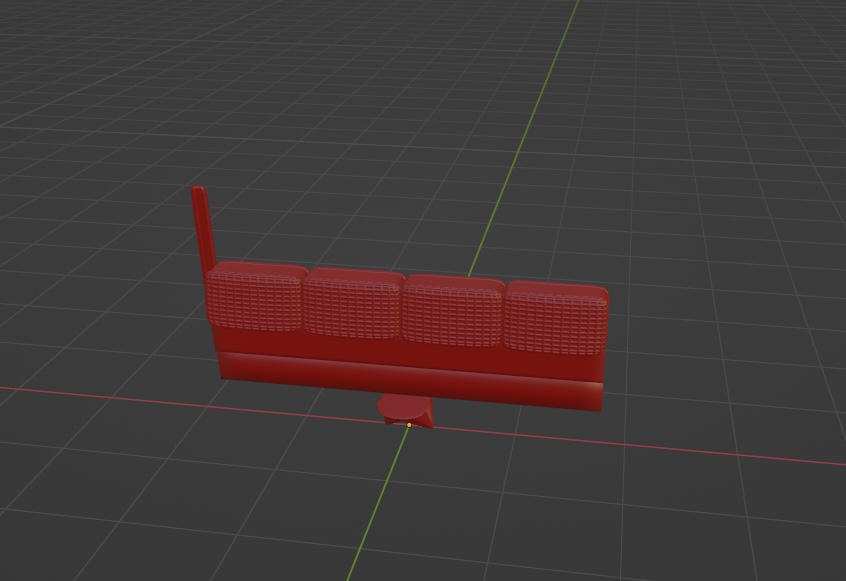
\includegraphics[scale=0.17]{./imgs/sofaParamMean/depthMin.png}
        \subcaption{Depth 最小(0.2)}
 \end{minipage}
 \begin{minipage}[b]{0.48\linewidth}
  \centering
  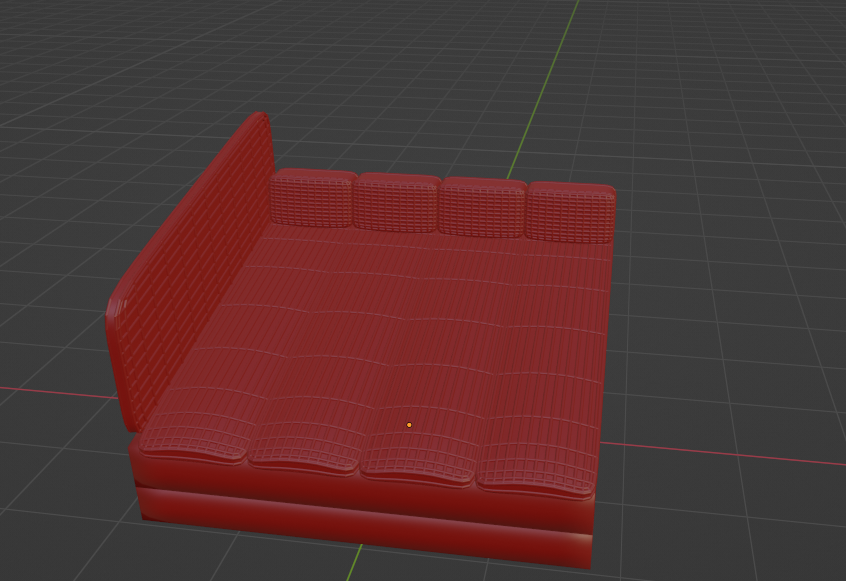
\includegraphics[scale=0.17]{./imgs/sofaParamMean/depthMax.png}
        \subcaption{Depth 最大(4.0)}
 \end{minipage}\\
  \begin{minipage}[b]{0.48\linewidth}
  \centering
  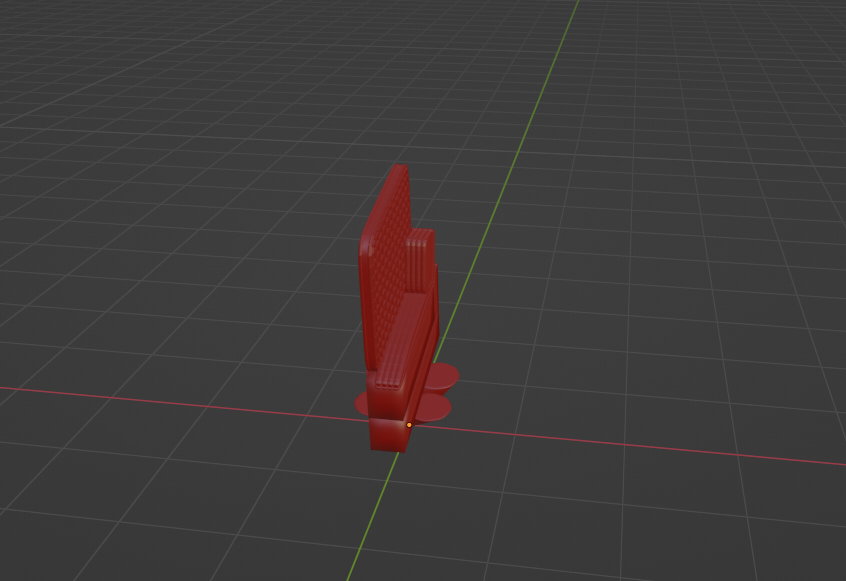
\includegraphics[scale=0.17]{./imgs/sofaParamMean/widthMin.png}
        \subcaption{Width 最小(0.3)}
 \end{minipage}
 \begin{minipage}[b]{0.48\linewidth}
  \centering
  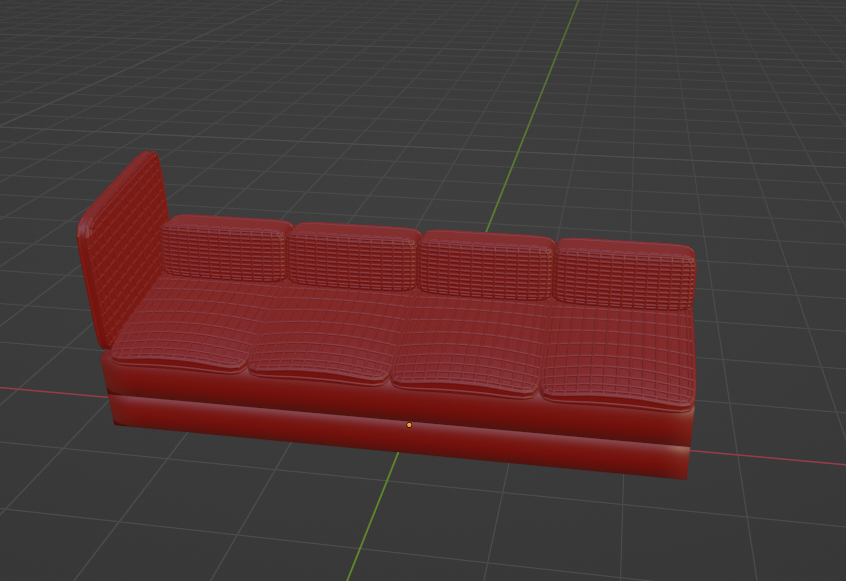
\includegraphics[scale=0.17]{./imgs/sofaParamMean/widthMax.png}
        \subcaption{Width 最大(5.0)}
 \end{minipage}\\
 \begin{minipage}[b]{0.48\linewidth}
  \centering
  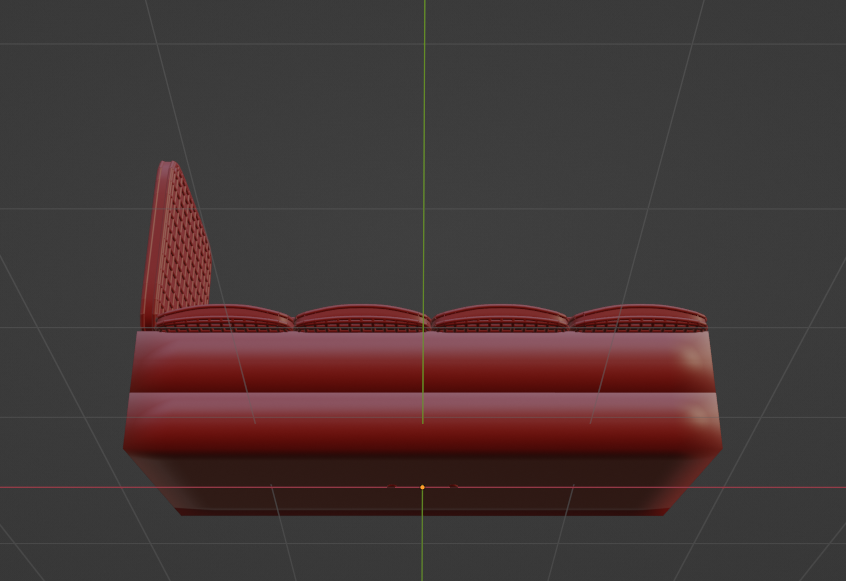
\includegraphics[scale=0.17]{./imgs/sofaParamMean/legHeightMin.png}
        \subcaption{Legs height 最小(0.01)}
 \end{minipage}
 \begin{minipage}[b]{0.48\linewidth}
  \centering
  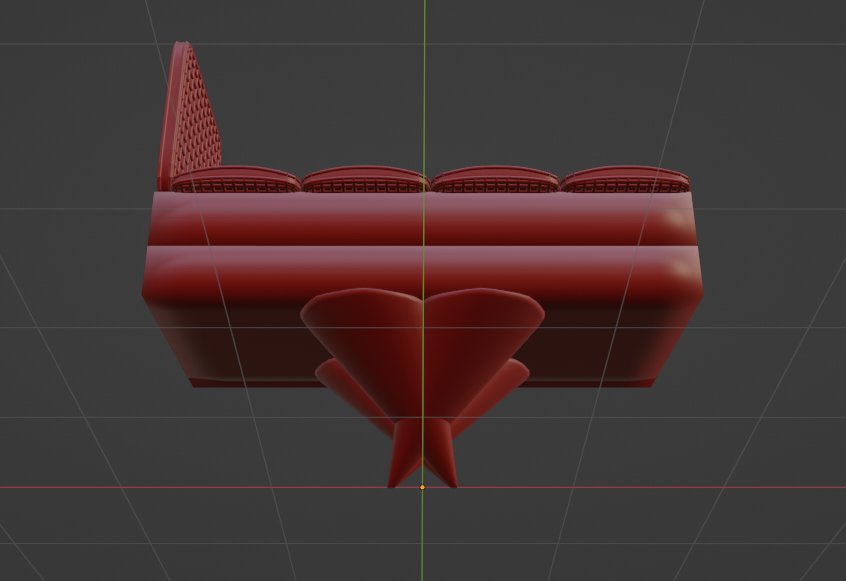
\includegraphics[scale=0.17]{./imgs/sofaParamMean/legHeightMax.png}
        \subcaption{Legs height 最大(1.0)}
 \end{minipage}\\
  \begin{minipage}[b]{0.48\linewidth}
  \centering
  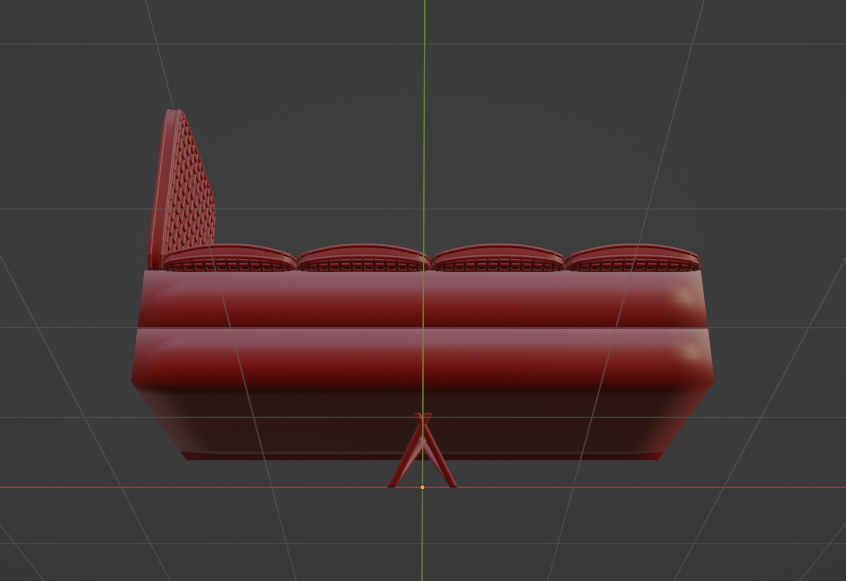
\includegraphics[scale=0.17]{./imgs/sofaParamMean/legShapeMin.png}
        \subcaption{Leg shape 最小(0.0)}
 \end{minipage}
 \begin{minipage}[b]{0.48\linewidth}
  \centering
  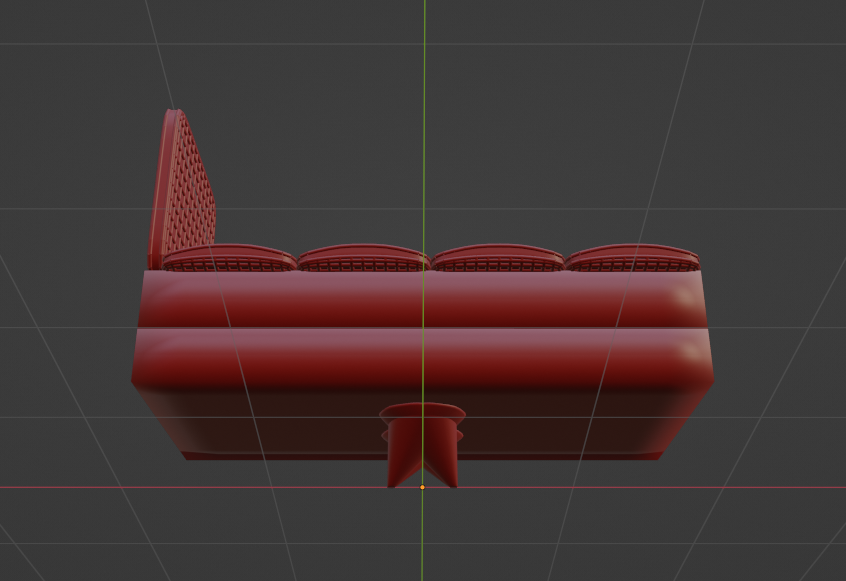
\includegraphics[scale=0.17]{./imgs/sofaParamMean/legShapeMax.png}
        \subcaption{Leg shape 最大(20.0)}
 \end{minipage}
 \caption{Sofa モデルにおけるパラメータ範囲(1)}\label{fig:sofaParamMean_1}
\end{figure}


\begin{figure}[h]
 \begin{minipage}[b]{0.48\linewidth}
  \centering
  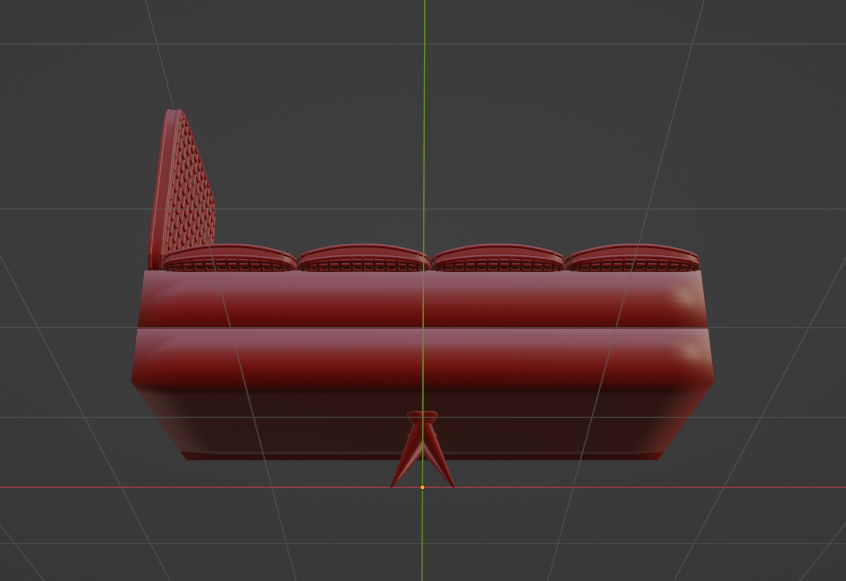
\includegraphics[scale=0.17]{./imgs/sofaParamMean/legDiameterMin.png}
        \subcaption{Leg diameter 最小(0.01)}
 \end{minipage}
 \begin{minipage}[b]{0.48\linewidth}
  \centering
  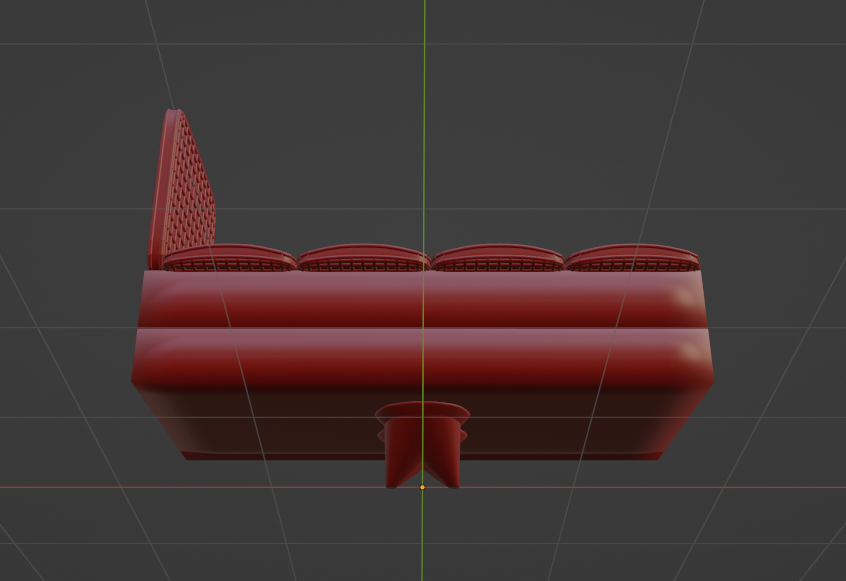
\includegraphics[scale=0.17]{./imgs/sofaParamMean/legDiameterMax.png}
        \subcaption{Leg diameter 最大(0.04)}
 \end{minipage}\\
 \begin{minipage}[b]{0.48\linewidth}
  \centering
  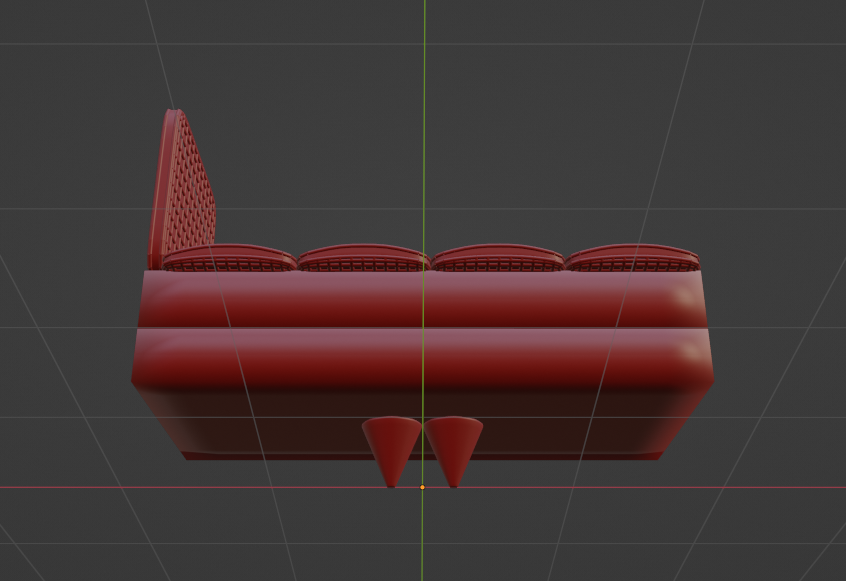
\includegraphics[scale=0.17]{./imgs/sofaParamMean/legAngleMin.png}
        \subcaption{Leg angle 最小(0.0)}
 \end{minipage}
 \begin{minipage}[b]{0.48\linewidth}
  \centering
  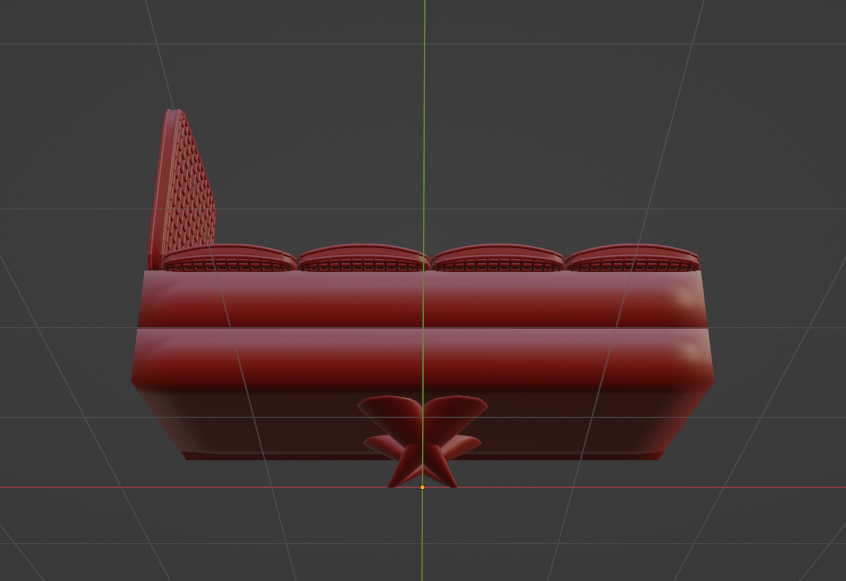
\includegraphics[scale=0.17]{./imgs/sofaParamMean/legAngleMax.png}
        \subcaption{Leg angle 最大(1.0)}
 \end{minipage}\\
  \begin{minipage}[b]{0.48\linewidth}
  \centering
  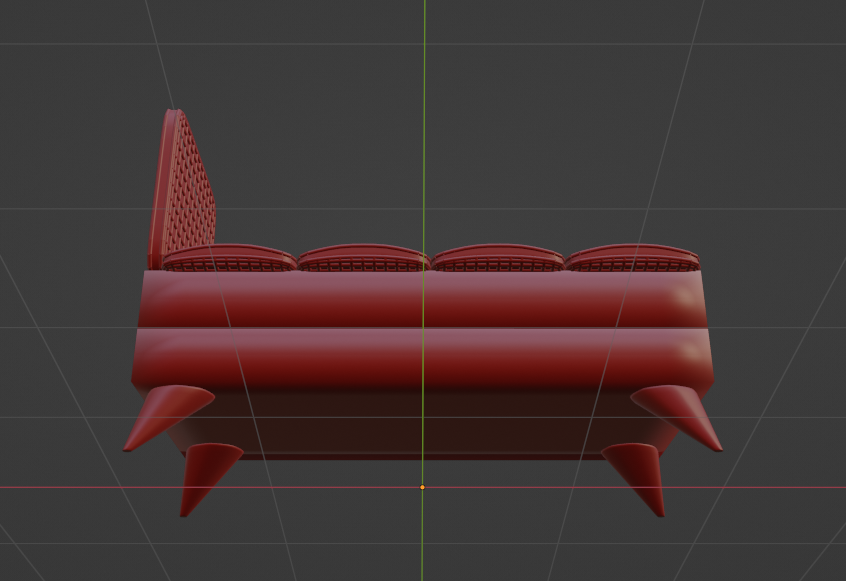
\includegraphics[scale=0.17]{./imgs/sofaParamMean/legPosMin.png}
        \subcaption{Leg position 最小(0.02)}
 \end{minipage}
 \begin{minipage}[b]{0.48\linewidth}
  \centering
  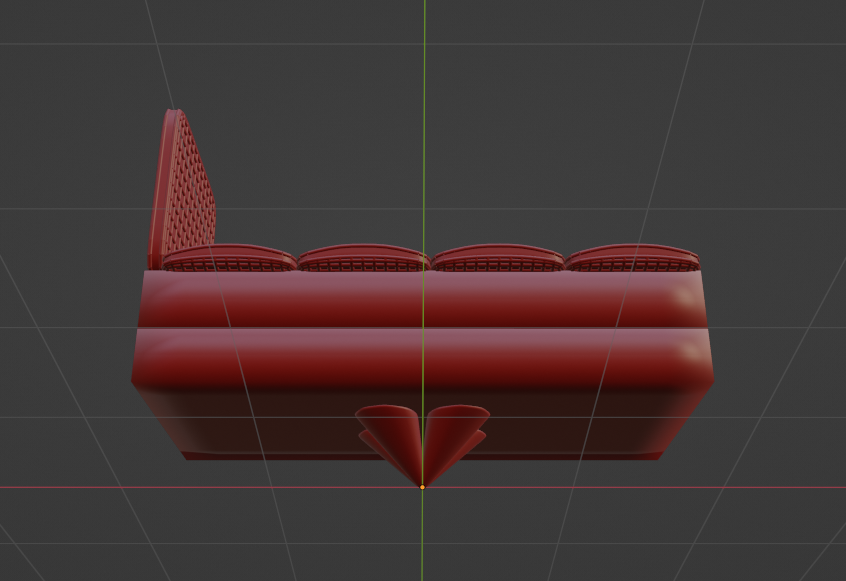
\includegraphics[scale=0.17]{./imgs/sofaParamMean/legPosMax.png}
        \subcaption{Leg position 最大(5.0)}
 \end{minipage}\\
 \begin{minipage}[b]{0.48\linewidth}
  \centering
  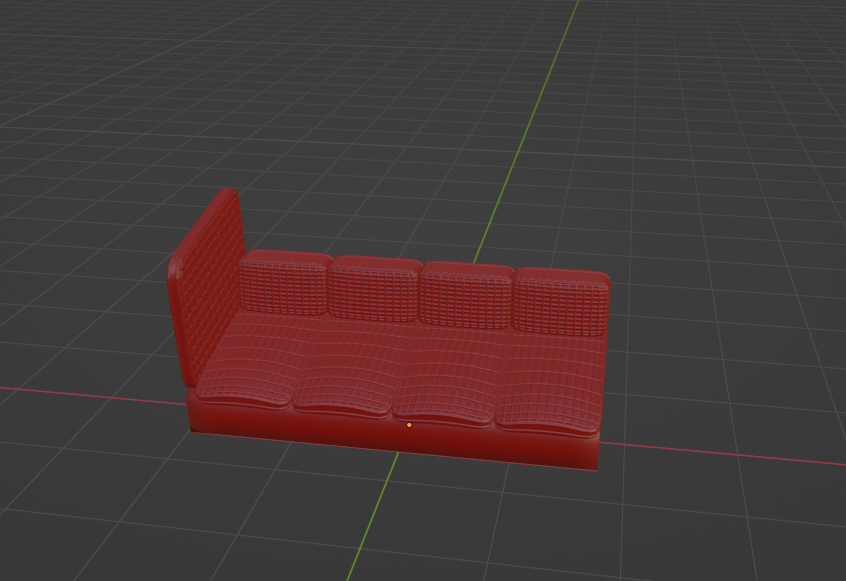
\includegraphics[scale=0.17]{./imgs/sofaParamMean/1BaseMin.png}
        \subcaption{Base height 最小(0.01)}
 \end{minipage}
 \begin{minipage}[b]{0.48\linewidth}
  \centering
  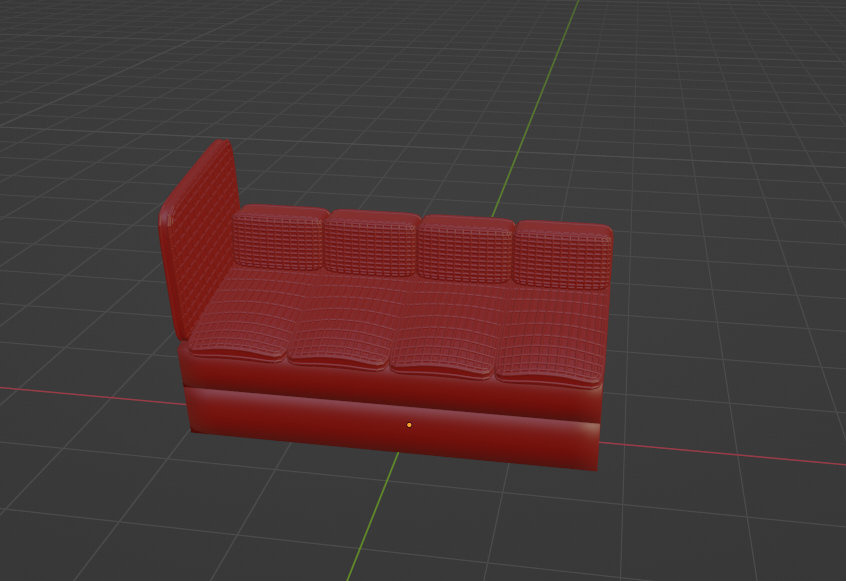
\includegraphics[scale=0.17]{./imgs/sofaParamMean/1BaseMax.png}
        \subcaption{Base height 最大(0.5)}
 \end{minipage}
 \caption{Sofa モデルにおけるパラメータ範囲(2)}\label{fig:sofaParamMean_2}
\end{figure}


\begin{figure}[h]
 \begin{minipage}[b]{0.48\linewidth}
  \centering
  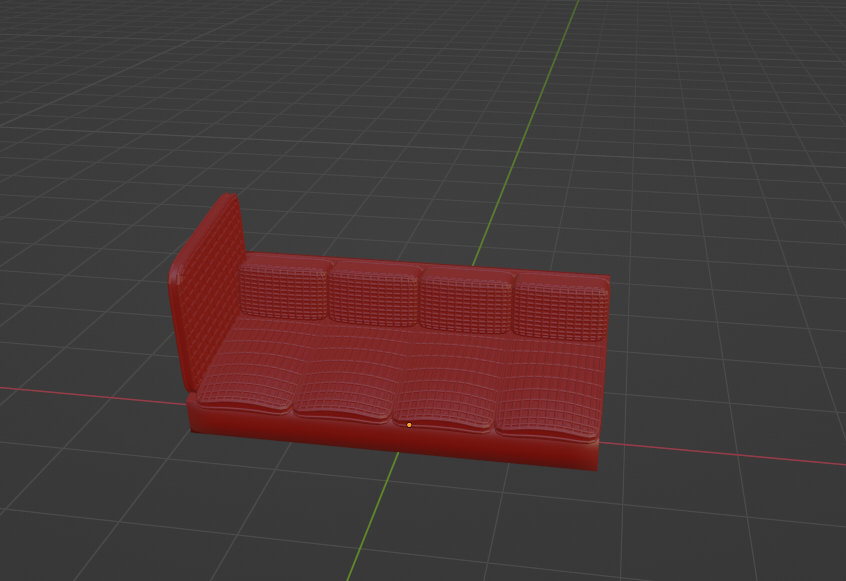
\includegraphics[scale=0.17]{./imgs/sofaParamMean/Base2HeightMin.png}
        \subcaption{Base2 height 最小(0.01)}
 \end{minipage}
 \begin{minipage}[b]{0.48\linewidth}
  \centering
  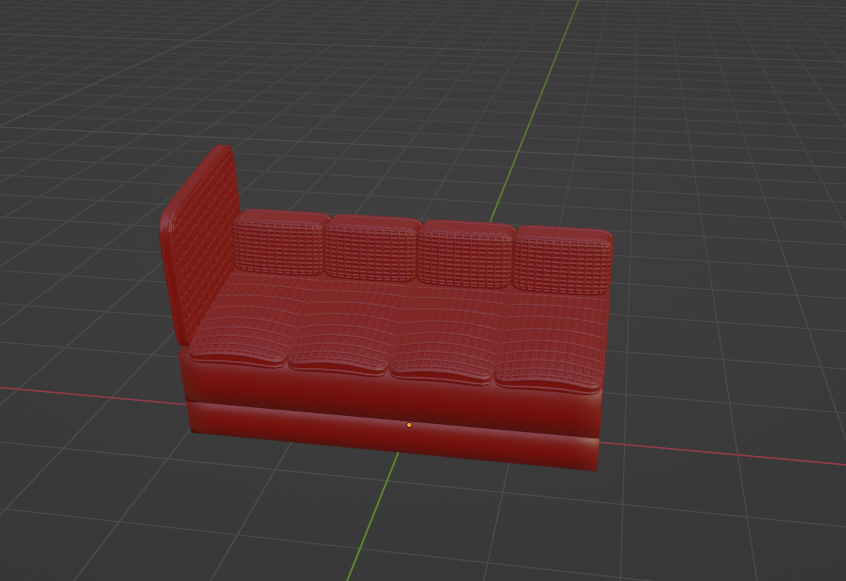
\includegraphics[scale=0.17]{./imgs/sofaParamMean/Base2HeightMax.png}
        \subcaption{Base2 height 最大(0.5)}
 \end{minipage}\\
 \begin{minipage}[b]{0.48\linewidth}
  \centering
  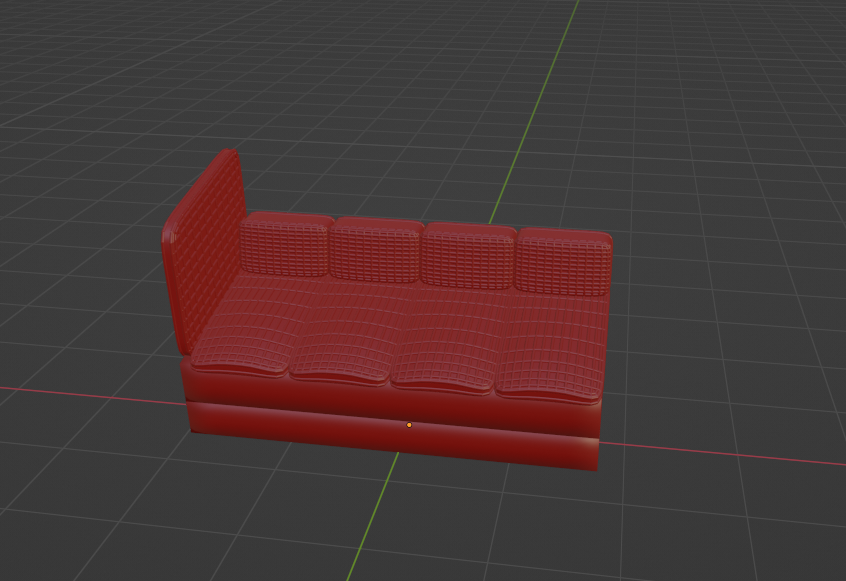
\includegraphics[scale=0.17]{./imgs/sofaParamMean/backTickMin.png}
        \subcaption{Back thickness 最小(0.01)}
 \end{minipage}
 \begin{minipage}[b]{0.48\linewidth}
  \centering
  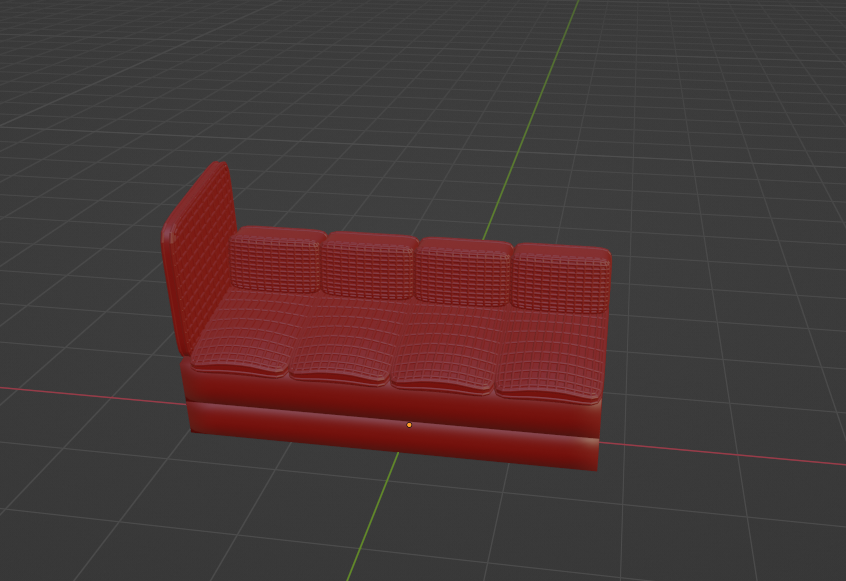
\includegraphics[scale=0.17]{./imgs/sofaParamMean/backTickMax.png}
        \subcaption{Back thickness 最大(0.3)}
 \end{minipage}\\
  \begin{minipage}[b]{0.48\linewidth}
  \centering
  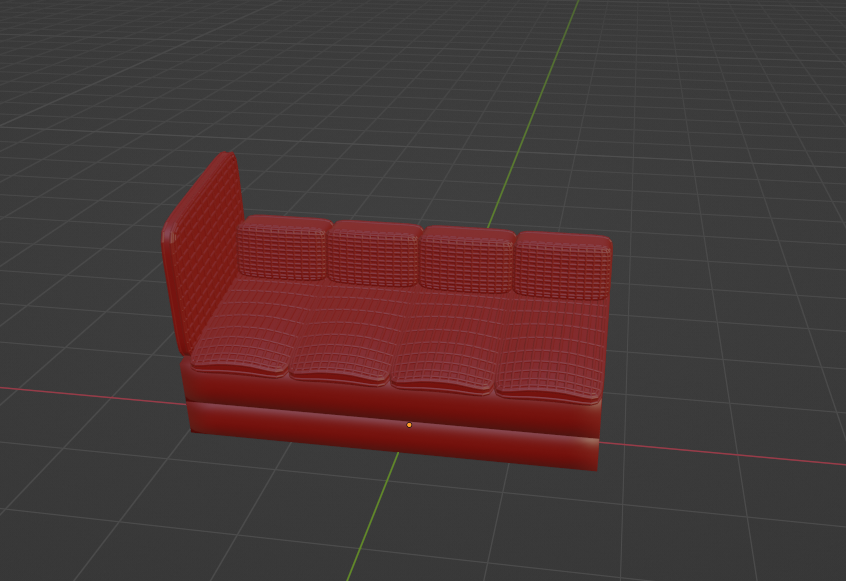
\includegraphics[scale=0.17]{./imgs/sofaParamMean/backSideHeightMin.png}
        \subcaption{Back/Side height 最小(0.01)}
 \end{minipage}
 \begin{minipage}[b]{0.48\linewidth}
  \centering
  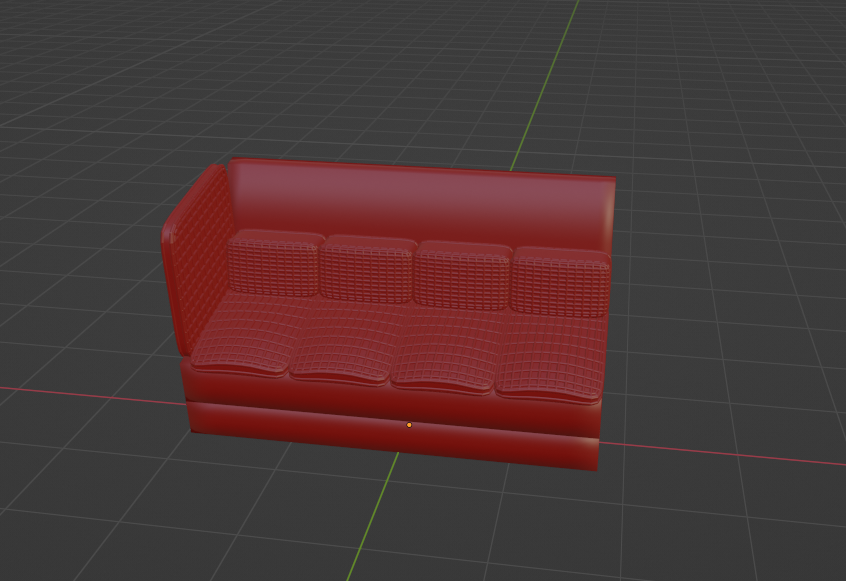
\includegraphics[scale=0.17]{./imgs/sofaParamMean/backSideHeightMax.png}
        \subcaption{Back/Side height 最大(1.5)}
 \end{minipage}\\
 \begin{minipage}[b]{0.48\linewidth}
  \centering
  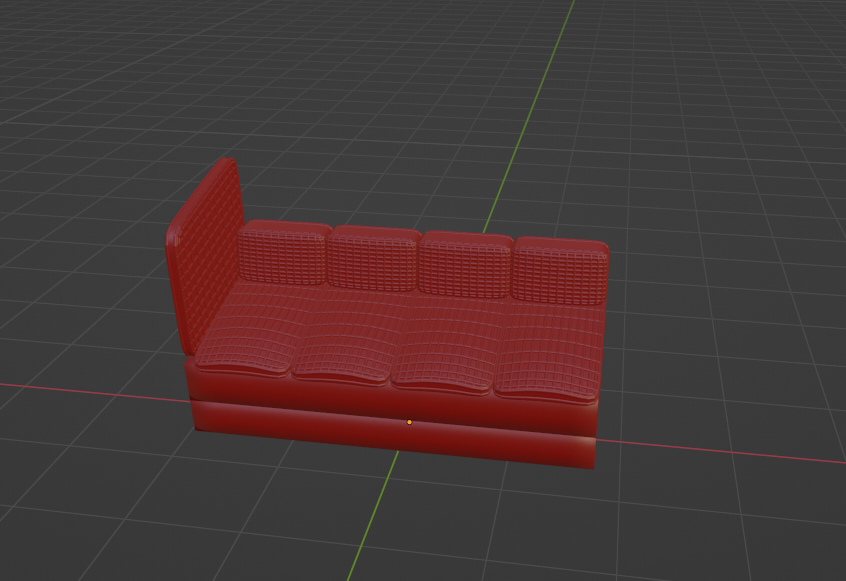
\includegraphics[scale=0.17]{./imgs/sofaParamMean/sideNumMin.png}
        \subcaption{Side NO / 1 / YES 最小(0)}
 \end{minipage}
 \begin{minipage}[b]{0.48\linewidth}
  \centering
  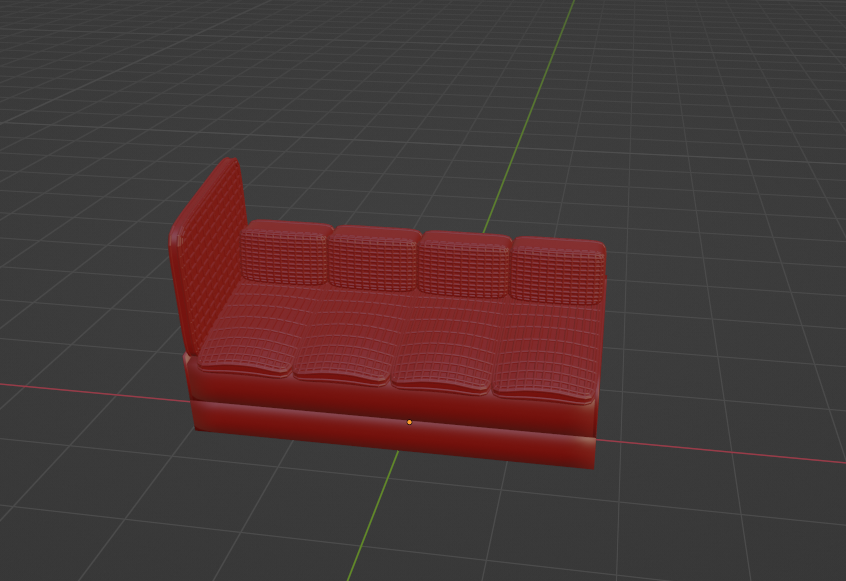
\includegraphics[scale=0.17]{./imgs/sofaParamMean/sideNumMax.png}
        \subcaption{Side NO / 1 / YES 最大(2)}
 \end{minipage}
 \caption{Sofa モデルにおけるパラメータ範囲(3)}\label{fig:sofaParamMean_3}
\end{figure}


\begin{figure}[h]
 \begin{minipage}[b]{0.48\linewidth}
  \centering
  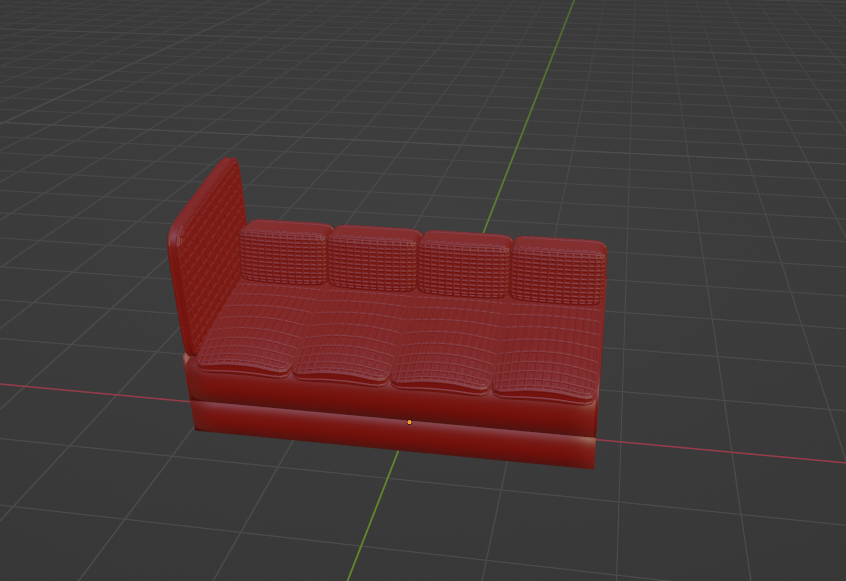
\includegraphics[scale=0.17]{./imgs/sofaParamMean/sideTicknessMin.png}
        \subcaption{Side thickness 最小(0.02)}
 \end{minipage}
 \begin{minipage}[b]{0.48\linewidth}
  \centering
  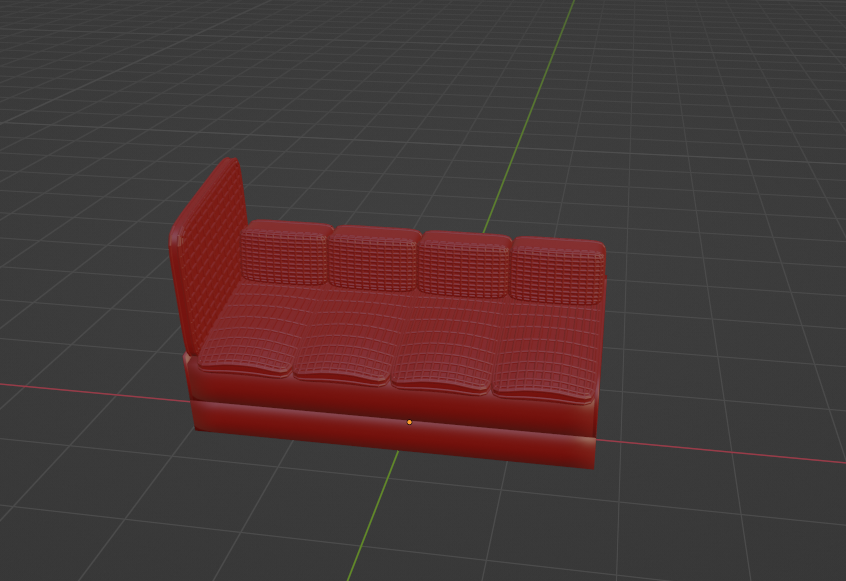
\includegraphics[scale=0.17]{./imgs/sofaParamMean/sideTicknessMax.png}
        \subcaption{Side thickness 最大(0.03)}
 \end{minipage}\\
 \begin{minipage}[b]{0.48\linewidth}
  \centering
  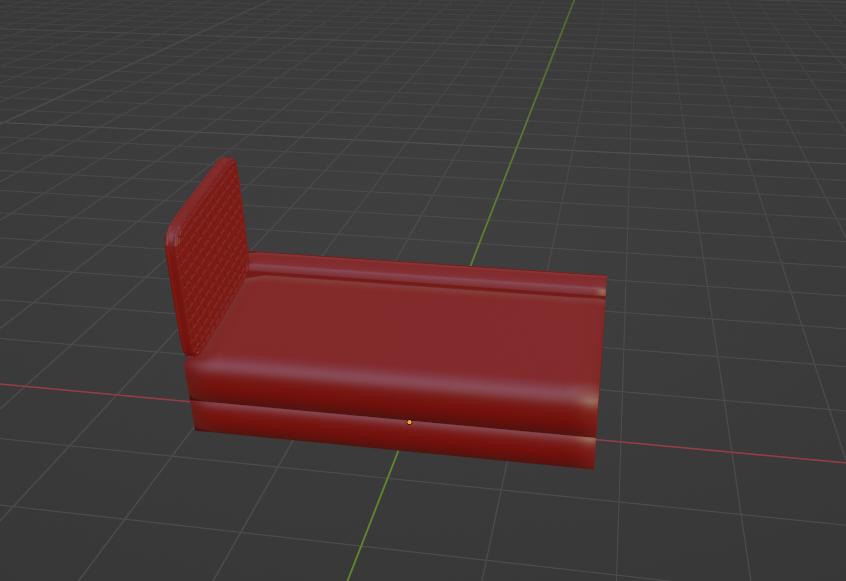
\includegraphics[scale=0.17]{./imgs/sofaParamMean/numCushionMin.png}
        \subcaption{N. of Cushions 最小(0)}
 \end{minipage}
 \begin{minipage}[b]{0.48\linewidth}
  \centering
  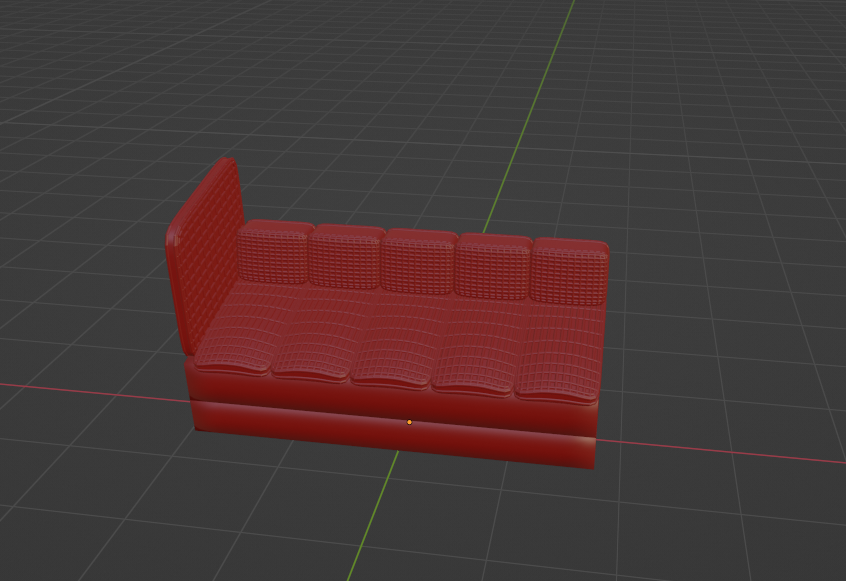
\includegraphics[scale=0.17]{./imgs/sofaParamMean/numCushionMax.png}
        \subcaption{N. of Cushions 最大(5)}
 \end{minipage}\\
  \begin{minipage}[b]{0.48\linewidth}
  \centering
  \includegraphics[scale=0.17]{./imgs/sofaParamMean/cushionTicknessMin.png}
        \subcaption{Cushion thickness 最小(0.05)}
 \end{minipage}
 \begin{minipage}[b]{0.48\linewidth}
  \centering
  \includegraphics[scale=0.17]{./imgs/sofaParamMean/cushionTicknessMax.png}
        \subcaption{Cushion thickness 最大(0.5)}
 \end{minipage}\\
 \begin{minipage}[b]{0.48\linewidth}
  \centering
  \includegraphics[scale=0.17]{./imgs/sofaParamMean/cushionNosingMin.png}
        \subcaption{Cushion nosing 最小(0.0)}
 \end{minipage}
 \begin{minipage}[b]{0.48\linewidth}
  \centering
  \includegraphics[scale=0.17]{./imgs/sofaParamMean/cushinoNosingMax.png}
        \subcaption{Cushion nosing 最大(0.3)}
 \end{minipage}
 \caption{Sofa モデルにおけるパラメータ範囲(4)}\label{fig:sofaParamMean_4}
\end{figure}


\begin{figure}[h]
 \begin{minipage}[b]{0.48\linewidth}
  \centering
  \includegraphics[scale=0.17]{./imgs/sofaParamMean/backCushionHeightMin.png}
        \subcaption{Back Cushion height 最小(0.1)}
 \end{minipage}
 \begin{minipage}[b]{0.48\linewidth}
  \centering
  \includegraphics[scale=0.17]{./imgs/sofaParamMean/backCushionHeightMax.png}
        \subcaption{Back Cushion height 最大(0.7)}
 \end{minipage}\\
 \begin{minipage}[b]{0.48\linewidth}
  \centering
  \includegraphics[scale=0.17]{./imgs/sofaParamMean/backCushionTickMin.png}
        \subcaption{Back Cush. Thickness / *Puffiness 最小(0.05)}
 \end{minipage}
 \begin{minipage}[b]{0.48\linewidth}
  \centering
  \includegraphics[scale=0.17]{./imgs/sofaParamMean/backCushionTickMax.png}
        \subcaption{Back Cush. Thickness / *Puffiness 最大(0.5)}
 \end{minipage}\\
  \begin{minipage}[b]{0.48\linewidth}
  \centering
  \includegraphics[scale=0.17]{./imgs/sofaParamMean/sideNumMin.png}
        \subcaption{Side Cushions NO / 1 / YES 最小(0)}
 \end{minipage}
 \begin{minipage}[b]{0.48\linewidth}
  \centering
  \includegraphics[scale=0.17]{./imgs/sofaParamMean/sideNumMax.png}
        \subcaption{Side Cushions NO / 1 / YES 最大(2)}
 \end{minipage}\\
 \begin{minipage}[b]{0.48\linewidth}
  \centering
  \includegraphics[scale=0.17]{./imgs/sofaParamMean/sideCushionHeightMin.png}
        \subcaption{Side Cushion Height 最小(0.1)}
 \end{minipage}
 \begin{minipage}[b]{0.48\linewidth}
  \centering
  \includegraphics[scale=0.17]{./imgs/sofaParamMean/sideCushionHeightMax.png}
        \subcaption{Side Cushion Height 最大(1.8)}
 \end{minipage}
 \caption{Sofa モデルにおけるパラメータ範囲(5)}\label{fig:sofaParamMean_5}
\end{figure}



\begin{figure}[h]
 \begin{minipage}[b]{0.48\linewidth}
  \centering
  \includegraphics[scale=0.17]{./imgs/sofaParamMean/sideCushionTickMin.png}
        \subcaption{Side Cushion Thickness 最小(0.0)}
 \end{minipage}
 \begin{minipage}[b]{0.48\linewidth}
  \centering
  \includegraphics[scale=0.17]{./imgs/sofaParamMean/sideCushionTickMax.png}
        \subcaption{Side Cushion Thickness 最大(0.05)}
 \end{minipage}\\
 \begin{minipage}[b]{0.48\linewidth}
  \centering
  \includegraphics[scale=0.17]{./imgs/sofaParamMean/stichingMin.png}
        \subcaption{Cushion Stitching 最小(0.0)}
 \end{minipage}
 \begin{minipage}[b]{0.48\linewidth}
  \centering
  \includegraphics[scale=0.17]{./imgs/sofaParamMean/stichingMax.png}
        \subcaption{Cushion Stitching 最大(0.05)}
 \end{minipage}\\
  \begin{minipage}[b]{0.48\linewidth}
  \centering
  \includegraphics[scale=0.17]{./imgs/sofaParamMean/creaseMin.png}
        \subcaption{Cushion Crease 最小(0.0)}
 \end{minipage}
 \begin{minipage}[b]{0.48\linewidth}
  \centering
  \includegraphics[scale=0.17]{./imgs/sofaParamMean/creaseMax.png}
        \subcaption{Cushion Crease 最大(0.3)}
 \end{minipage}\\
 \begin{minipage}[b]{0.48\linewidth}
  \centering
  \includegraphics[scale=0.17]{./imgs/sofaParamMean/bevelMin.png}
        \subcaption{Bevel 最小(0.001)}
 \end{minipage}
 \begin{minipage}[b]{0.48\linewidth}
  \centering
  \includegraphics[scale=0.17]{./imgs/sofaParamMean/bevelMax.png}
        \subcaption{Bevel 最大(1.0)}
 \end{minipage}
 \caption{Sofa モデルにおけるパラメータ範囲(6)}\label{fig:sofaParamMean_6}
\end{figure}



\begin{figure}[h]
 \begin{minipage}[b]{0.48\linewidth}
  \centering
  \includegraphics[scale=0.17]{./imgs/sofaParamMean/subdMin.png}
        \subcaption{Subd 最小(0)}
 \end{minipage}
 \begin{minipage}[b]{0.48\linewidth}
  \centering
  \includegraphics[scale=0.17]{./imgs/sofaParamMean/subdMax.png}
        \subcaption{Subd 最大(2)}
 \end{minipage}
 \caption{Sofa モデルにおけるパラメータ範囲(7)}\label{fig:sofaParamMean_7}
\end{figure}

\clearpage

\setcounter{table}{0}
\setcounter{figure}{0}

\section{提案モデルの推移}\label{appendix:gaChange}
本付録では,遺伝的アルゴリズムの推移を具体的なグラフを用いて示す.
図\ref{fig:gaChange1_1} - \ref{fig:gaChange1_3}に
実験1における具体的な提案モデルの推移を,
図\ref{fig:gaChange2_1} - \ref{fig:gaChange2_3}に
実験2における具体的な提案モデルの推移を示す.
既存の研究では縦軸は適応度が利用されるが,本研究では選択によって行われるため実験1では見本モデルとの,実験2では最後に作成されたモデルとのユークリッド距離を用いる.この時,各遺伝子の定義域について Min - Max normalization を事前処理として行っている.また,箱ひげ図が各ステップの提案モデル群,折れ線グラフが次ステップに進む前に決定されたモデルを意味する.

\begin{figure}[h]
 \begin{minipage}[b]{0.48\linewidth}
  \centering
  \includegraphics[scale=0.15]{./imgs/gaChange/cake1_1.pdf}
        \subcaption{被験者1,提案システム}
 \end{minipage}
 \begin{minipage}[b]{0.48\linewidth}
  \centering
  \includegraphics[scale=0.15]{./imgs/gaChange/cake2_1.pdf}
        \subcaption{被験者1,既存システム}
 \end{minipage}\\
 \begin{minipage}[b]{0.48\linewidth}
  \centering
  \includegraphics[scale=0.15]{./imgs/gaChange/cake1_2.pdf}
        \subcaption{被験者2,提案システム}
 \end{minipage}
 \begin{minipage}[b]{0.48\linewidth}
  \centering
  \includegraphics[scale=0.15]{./imgs/gaChange/cake2_2.pdf}
        \subcaption{被験者2,既存システム}
 \end{minipage}\\
 \begin{minipage}[b]{0.48\linewidth}
  \centering
  \includegraphics[scale=0.15]{./imgs/gaChange/cake1_3.pdf}
        \subcaption{被験者3,提案システム}
 \end{minipage}
 \begin{minipage}[b]{0.48\linewidth}
  \centering
  \includegraphics[scale=0.15]{./imgs/gaChange/cake2_3.pdf}
        \subcaption{被験者3,既存システム}
 \end{minipage}\\
 \begin{minipage}[b]{0.48\linewidth}
  \centering
  \includegraphics[scale=0.15]{./imgs/gaChange/cake1_4.pdf}
        \subcaption{被験者4,提案システム}
 \end{minipage}
 \begin{minipage}[b]{0.48\linewidth}
  \centering
  \includegraphics[scale=0.15]{./imgs/gaChange/cake2_4.pdf}
        \subcaption{被験者4,既存システム}
 \end{minipage}
 \caption{実験1における提案モデルの推移(1)}\label{fig:gaChange1_1}
\end{figure}

\begin{figure}[h]
 \begin{minipage}[b]{0.48\linewidth}
  \centering
  \includegraphics[scale=0.15]{./imgs/gaChange/cake1_5.pdf}
        \subcaption{被験者5,提案システム}
 \end{minipage}
 \begin{minipage}[b]{0.48\linewidth}
  \centering
  \includegraphics[scale=0.15]{./imgs/gaChange/cake2_5.pdf}
        \subcaption{被験者5,既存システム}
 \end{minipage}\\
 \begin{minipage}[b]{0.48\linewidth}
  \centering
  \includegraphics[scale=0.15]{./imgs/gaChange/cake1_6.pdf}
        \subcaption{被験者6,提案システム}
 \end{minipage}
 \begin{minipage}[b]{0.48\linewidth}
  \centering
  \includegraphics[scale=0.15]{./imgs/gaChange/cake2_6.pdf}
        \subcaption{被験者6,既存システム}
 \end{minipage}\\
 \begin{minipage}[b]{0.48\linewidth}
  \centering
  \includegraphics[scale=0.15]{./imgs/gaChange/cake1_7.pdf}
        \subcaption{被験者7,提案システム}
 \end{minipage}
 \begin{minipage}[b]{0.48\linewidth}
  \centering
  \includegraphics[scale=0.15]{./imgs/gaChange/cake2_7.pdf}
        \subcaption{被験者7,既存システム}
 \end{minipage}\\
 \begin{minipage}[b]{0.48\linewidth}
  \centering
  \includegraphics[scale=0.15]{./imgs/gaChange/cake1_8.pdf}
        \subcaption{被験者8,提案システム}
 \end{minipage}
 \begin{minipage}[b]{0.48\linewidth}
  \centering
  \includegraphics[scale=0.15]{./imgs/gaChange/cake2_8.pdf}
        \subcaption{被験者8,既存システム}
 \end{minipage}
 \caption{実験1における提案モデルの推移(2)}\label{fig:gaChange1_2}
\end{figure}

\begin{figure}[h]
 \begin{minipage}[b]{0.48\linewidth}
  \centering
  \includegraphics[scale=0.15]{./imgs/gaChange/cake1_9.pdf}
        \subcaption{被験者9,提案システム}
 \end{minipage}
 \begin{minipage}[b]{0.48\linewidth}
  \centering
  \includegraphics[scale=0.15]{./imgs/gaChange/cake2_9.pdf}
        \subcaption{被験者9,既存システム}
 \end{minipage}\\
 \begin{minipage}[b]{0.48\linewidth}
  \centering
  \includegraphics[scale=0.15]{./imgs/gaChange/cake1_10.pdf}
        \subcaption{被験者10,提案システム}
 \end{minipage}
 \begin{minipage}[b]{0.48\linewidth}
  \centering
  \includegraphics[scale=0.15]{./imgs/gaChange/cake2_10.pdf}
        \subcaption{被験者10,既存システム}
 \end{minipage}\\
 \begin{minipage}[b]{0.48\linewidth}
  \centering
  \includegraphics[scale=0.15]{./imgs/gaChange/cake1_11.pdf}
        \subcaption{被験者11,提案システム}
 \end{minipage}
 \begin{minipage}[b]{0.48\linewidth}
  \centering
  \includegraphics[scale=0.15]{./imgs/gaChange/cake2_11.pdf}
        \subcaption{被験者11,既存システム}
 \end{minipage}
 \caption{実験1における提案モデルの推移(3)}\label{fig:gaChange1_3}
\end{figure}

\begin{figure}[h]
 \begin{minipage}[b]{0.48\linewidth}
  \centering
  \includegraphics[scale=0.15]{./imgs/gaChange/sofa1_1.pdf}
        \subcaption{被験者1,提案システム}
 \end{minipage}
 \begin{minipage}[b]{0.48\linewidth}
  \centering
  \includegraphics[scale=0.15]{./imgs/gaChange/sofa2_1.pdf}
        \subcaption{被験者1,既存システム}
 \end{minipage}\\
 \begin{minipage}[b]{0.48\linewidth}
  \centering
  \includegraphics[scale=0.15]{./imgs/gaChange/sofa1_2.pdf}
        \subcaption{被験者2,提案システム}
 \end{minipage}
 \begin{minipage}[b]{0.48\linewidth}
  \centering
  \includegraphics[scale=0.15]{./imgs/gaChange/sofa2_2.pdf}
        \subcaption{被験者2,既存システム}
 \end{minipage}\\
 \begin{minipage}[b]{0.48\linewidth}
  \centering
  \includegraphics[scale=0.15]{./imgs/gaChange/sofa1_3.pdf}
        \subcaption{被験者3,提案システム}
 \end{minipage}
 \begin{minipage}[b]{0.48\linewidth}
  \centering
  \includegraphics[scale=0.15]{./imgs/gaChange/sofa2_3.pdf}
        \subcaption{被験者3,既存システム}
 \end{minipage}\\
 \begin{minipage}[b]{0.48\linewidth}
  \centering
  \includegraphics[scale=0.15]{./imgs/gaChange/sofa1_4.pdf}
        \subcaption{被験者4,提案システム}
 \end{minipage}
 \begin{minipage}[b]{0.48\linewidth}
  \centering
  \includegraphics[scale=0.15]{./imgs/gaChange/sofa2_4.pdf}
        \subcaption{被験者4,既存システム}
 \end{minipage}
 \caption{実験2における提案モデルの推移(1)}\label{fig:gaChange2_1}
\end{figure}

\begin{figure}[h]
 \begin{minipage}[b]{0.48\linewidth}
  \centering
  \includegraphics[scale=0.15]{./imgs/gaChange/sofa1_5.pdf}
        \subcaption{被験者5,提案システム}
 \end{minipage}
 \begin{minipage}[b]{0.48\linewidth}
  \centering
  \includegraphics[scale=0.15]{./imgs/gaChange/sofa2_5.pdf}
        \subcaption{被験者5,既存システム}
 \end{minipage}\\
 \begin{minipage}[b]{0.48\linewidth}
  \centering
  \includegraphics[scale=0.15]{./imgs/gaChange/sofa1_6.pdf}
        \subcaption{被験者6,提案システム}
 \end{minipage}
 \begin{minipage}[b]{0.48\linewidth}
  \centering
  \includegraphics[scale=0.15]{./imgs/gaChange/sofa2_6.pdf}
        \subcaption{被験者6,既存システム}
 \end{minipage}\\
 \begin{minipage}[b]{0.48\linewidth}
  \centering
  \includegraphics[scale=0.15]{./imgs/gaChange/sofa1_7.pdf}
        \subcaption{被験者7,提案システム}
 \end{minipage}
 \begin{minipage}[b]{0.48\linewidth}
  \centering
  \includegraphics[scale=0.15]{./imgs/gaChange/sofa2_7.pdf}
        \subcaption{被験者7,既存システム}
 \end{minipage}\\
 \begin{minipage}[b]{0.48\linewidth}
  \centering
  \includegraphics[scale=0.15]{./imgs/gaChange/sofa1_8.pdf}
        \subcaption{被験者8,提案システム}
 \end{minipage}
 \begin{minipage}[b]{0.48\linewidth}
  \centering
  \includegraphics[scale=0.15]{./imgs/gaChange/sofa2_8.pdf}
        \subcaption{被験者8,既存システム}
 \end{minipage}
 \caption{実験2における提案モデルの推移(2)}\label{fig:gaChange2_2}
\end{figure}

\begin{figure}[h]
 \begin{minipage}[b]{0.48\linewidth}
  \centering
  \includegraphics[scale=0.15]{./imgs/gaChange/sofa1_9.pdf}
        \subcaption{被験者9,提案システム}
 \end{minipage}
 \begin{minipage}[b]{0.48\linewidth}
  \centering
  \includegraphics[scale=0.15]{./imgs/gaChange/sofa2_9.pdf}
        \subcaption{被験者9,既存システム}
 \end{minipage}\\
 \begin{minipage}[b]{0.48\linewidth}
  \centering
  \includegraphics[scale=0.15]{./imgs/gaChange/sofa1_10.pdf}
        \subcaption{被験者10,提案システム}
 \end{minipage}
 \begin{minipage}[b]{0.48\linewidth}
  \centering
  \includegraphics[scale=0.15]{./imgs/gaChange/sofa2_10.pdf}
        \subcaption{被験者10,既存システム}
 \end{minipage}\\
 \begin{minipage}[b]{0.48\linewidth}
  \centering
  \includegraphics[scale=0.15]{./imgs/gaChange/sofa1_11.pdf}
        \subcaption{被験者11,提案システム}
 \end{minipage}
 \begin{minipage}[b]{0.48\linewidth}
  \centering
  \includegraphics[scale=0.15]{./imgs/gaChange/sofa2_11.pdf}
        \subcaption{被験者11,既存システム}
 \end{minipage}
 \caption{実験3における提案モデルの推移(3)}\label{fig:gaChange2_3}
\end{figure}

\clearpage

\setcounter{table}{0}
\setcounter{figure}{0}

\section{提案モデルパラメータの二次元可視化}\label{appendix:tSNE}
\hyperref[appendix:gaChange]{付録B}で示した提案モデルの推移では,提案モデルパラメータを最終モデルとの距離によって視覚化したが、それだけでは探索範囲の比較が難しい.そこで本章では t-SNE \cite{van2008visualizing} という手法により二次元に次元削減を行う.
図\ref{fig:tSNE1_1},\ref{fig:tSNE1_2}に実験1を,図\ref{fig:tSNE2_1},\ref{fig:tSNE2_2}に実験2の結果を示す.
この散布図について縁取りが青いものが提案システム,赤いものが既存システムによる提案モデルであり,内部の色が0から1に行くにつれてステップ数が増加するようにしている. また,軸についてはそれぞれ無次元量である.

\begin{figure}[h]
 \begin{minipage}[b]{0.48\linewidth}
  \centering
  \includegraphics[scale=0.15]{./imgs/tSNE/cake_1.pdf}
        \subcaption{被験者1}
 \end{minipage}
 \begin{minipage}[b]{0.48\linewidth}
  \centering
  \includegraphics[scale=0.15]{./imgs/tSNE/cake_2.pdf}
        \subcaption{被験者2}
 \end{minipage}\\
 \begin{minipage}[b]{0.48\linewidth}
  \centering
  \includegraphics[scale=0.15]{./imgs/tSNE/cake_3.pdf}
        \subcaption{被験者3}
 \end{minipage}
 \begin{minipage}[b]{0.48\linewidth}
  \centering
  \includegraphics[scale=0.15]{./imgs/tSNE/cake_4.pdf}
        \subcaption{被験者4}
 \end{minipage}\\
 \begin{minipage}[b]{0.48\linewidth}
  \centering
  \includegraphics[scale=0.15]{./imgs/tSNE/cake_5.pdf}
        \subcaption{被験者5}
 \end{minipage}
 \begin{minipage}[b]{0.48\linewidth}
  \centering
  \includegraphics[scale=0.15]{./imgs/tSNE/cake_6.pdf}
        \subcaption{被験者6}
 \end{minipage}\\
 \caption{実験1におけるパラメータの二次元可視化(1)}\label{fig:tSNE1_1}
\end{figure}

\begin{figure}[h]
 \begin{minipage}[b]{0.48\linewidth}
  \centering
  \includegraphics[scale=0.15]{./imgs/tSNE/cake_7.pdf}
        \subcaption{被験者7}
 \end{minipage}
 \begin{minipage}[b]{0.48\linewidth}
  \centering
  \includegraphics[scale=0.15]{./imgs/tSNE/cake_8.pdf}
        \subcaption{被験者8}
 \end{minipage}\\
 \begin{minipage}[b]{0.48\linewidth}
  \centering
  \includegraphics[scale=0.15]{./imgs/tSNE/cake_9.pdf}
        \subcaption{被験者9}
 \end{minipage}
 \begin{minipage}[b]{0.48\linewidth}
  \centering
  \includegraphics[scale=0.15]{./imgs/tSNE/cake_10.pdf}
        \subcaption{被験者10}
 \end{minipage}\\
 \begin{minipage}[b]{0.48\linewidth}
  \centering
  \includegraphics[scale=0.15]{./imgs/tSNE/cake_11.pdf}
        \subcaption{被験者11}
 \end{minipage}\\
 \caption{実験1におけるパラメータの二次元可視化(2)}\label{fig:tSNE1_2}
\end{figure}



\begin{figure}[h]
 \begin{minipage}[b]{0.48\linewidth}
  \centering
  \includegraphics[scale=0.15]{./imgs/tSNE/sofa_1.pdf}
        \subcaption{被験者1}
 \end{minipage}
 \begin{minipage}[b]{0.48\linewidth}
  \centering
  \includegraphics[scale=0.15]{./imgs/tSNE/sofa_2.pdf}
        \subcaption{被験者2}
 \end{minipage}\\
 \begin{minipage}[b]{0.48\linewidth}
  \centering
  \includegraphics[scale=0.15]{./imgs/tSNE/sofa_3.pdf}
        \subcaption{被験者3}
 \end{minipage}
 \begin{minipage}[b]{0.48\linewidth}
  \centering
  \includegraphics[scale=0.15]{./imgs/tSNE/sofa_4.pdf}
        \subcaption{被験者4}
 \end{minipage}\\
 \begin{minipage}[b]{0.48\linewidth}
  \centering
  \includegraphics[scale=0.15]{./imgs/tSNE/sofa_5.pdf}
        \subcaption{被験者5}
 \end{minipage}
 \begin{minipage}[b]{0.48\linewidth}
  \centering
  \includegraphics[scale=0.15]{./imgs/tSNE/sofa_6.pdf}
        \subcaption{被験者6}
 \end{minipage}\\
 \caption{実験2におけるパラメータの二次元可視化(1)}\label{fig:tSNE2_1}
\end{figure}

\begin{figure}[h]
 \begin{minipage}[b]{0.48\linewidth}
  \centering
  \includegraphics[scale=0.15]{./imgs/tSNE/sofa_7.pdf}
        \subcaption{被験者7}
 \end{minipage}
 \begin{minipage}[b]{0.48\linewidth}
  \centering
  \includegraphics[scale=0.15]{./imgs/tSNE/sofa_8.pdf}
        \subcaption{被験者8}
 \end{minipage}\\
 \begin{minipage}[b]{0.48\linewidth}
  \centering
  \includegraphics[scale=0.15]{./imgs/tSNE/sofa_9.pdf}
        \subcaption{被験者9}
 \end{minipage}
 \begin{minipage}[b]{0.48\linewidth}
  \centering
  \includegraphics[scale=0.15]{./imgs/tSNE/sofa_10.pdf}
        \subcaption{被験者10}
 \end{minipage}\\
 \begin{minipage}[b]{0.48\linewidth}
  \centering
  \includegraphics[scale=0.15]{./imgs/tSNE/sofa_11.pdf}
        \subcaption{被験者11}
 \end{minipage}\\
 \caption{実験2におけるパラメータの二次元可視化(2)}\label{fig:tSNE2_2}
\end{figure}